\section{Installation}
\subsection{System Requirements}
In order to install Librede, your system needs to meet the following prerequisites:
\begin{itemize}
\item \emph{Operation System:} Windows 7/8/10 32-bit or 64-bit, Linux 64-bit (MacOS X and Linux 32-bit are currently not supported)
\item \emph{Java Runtime Environment:} at least 1.6 (on Linux only 64-bit version supported)
\item \emph{Eclipse:} Eclipse Standard 4.4 or higher (download from \url{http://www.eclipse.org/downloads/})
\item \emph{Other:} On Linux please ensure that the library gfortran is installed. On Windows Librede comes with its own version.

\subsection{New Installation}
\end{itemize}

Your can install Librede in as an Eclipse plugin with an update site. Follow these steps:

\begin{itemize}
	\item In Eclipse go to menu "Help 	$ \rightarrow $ Install new Software" \newline
			\newline
			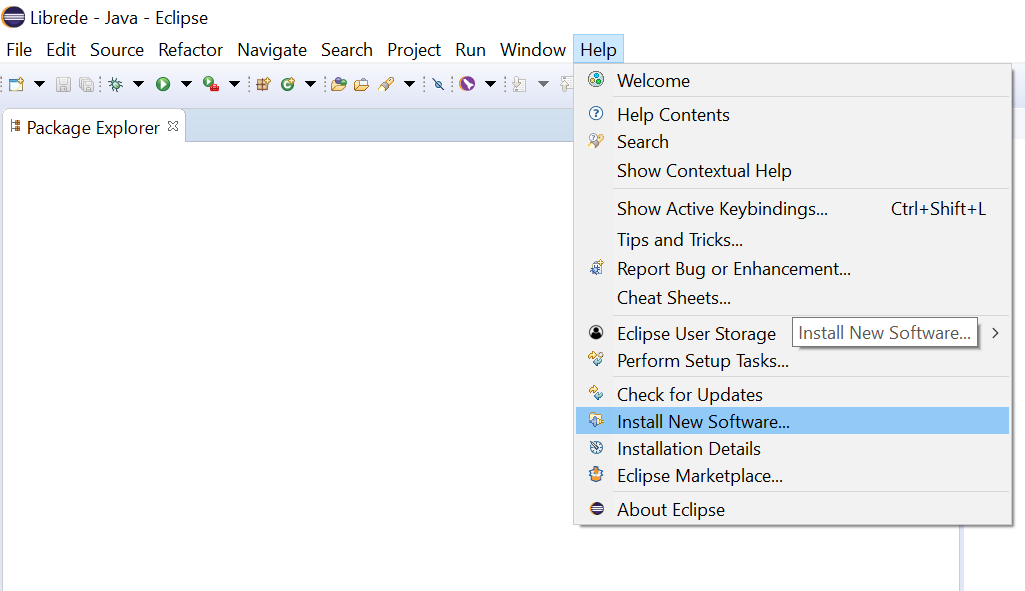
\includegraphics[width=0.9\textwidth]{screenshots/Screenshot3}
	
	\item Add a new repository with \url{https://se4.informatik.uni-wuerzburg.de/librede/downloads/snapshot/} as location.\newline
			\newline
			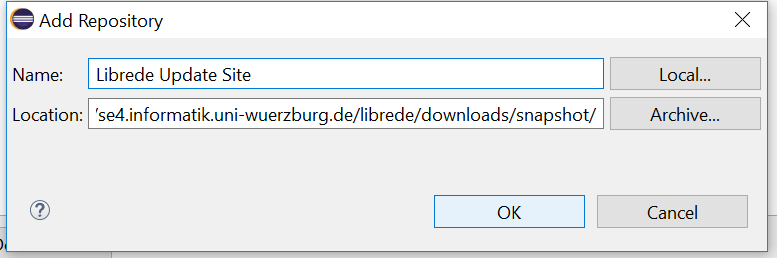
\includegraphics[width=0.6\textwidth]{screenshots/Screenshot5}
	\item Mark the Librede feature for installation and click next.
	\item Accept the license agreement.
	\item Confirm the security warning. \newline
			\newline
			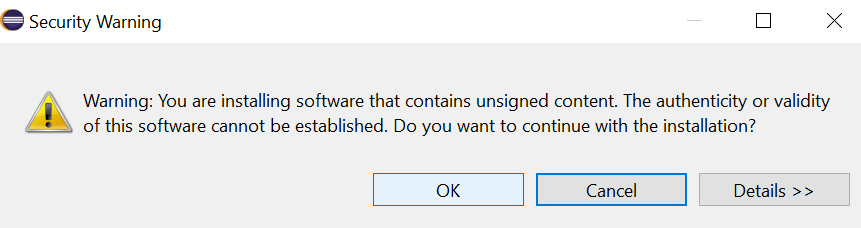
\includegraphics[width=0.6\textwidth]{screenshots/Screenshot6}
	\item After completion, restart Eclipse.
	
\end{itemize}

\subsection{Update Existing Installation}
To update an existing installation of the Librede Eclipse plugin follow these steps:

\begin{itemize}
	\item In Eclipse go to menu "Help $ \rightarrow $ Check for Updates" \newline
			\newline
			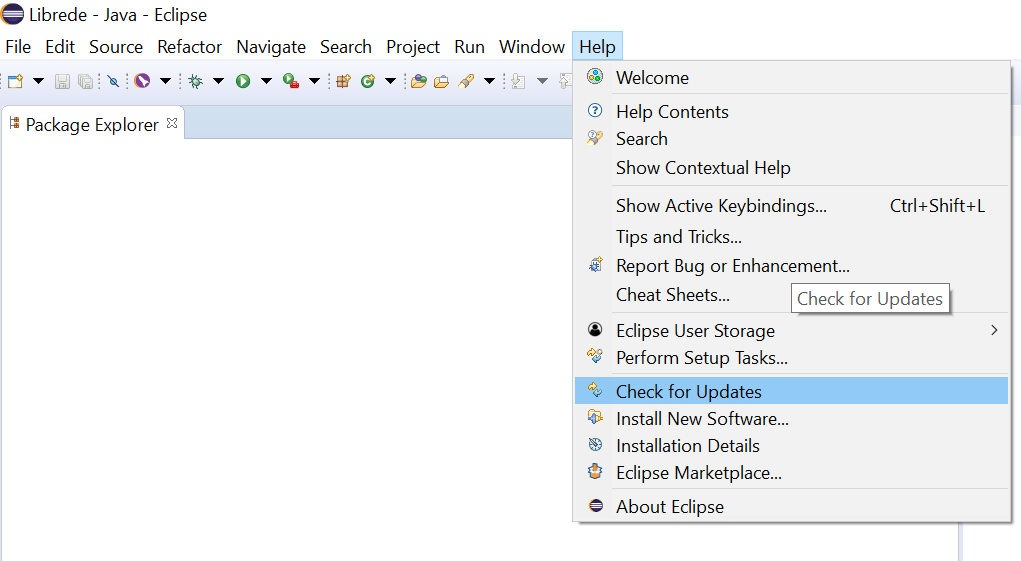
\includegraphics[width=0.9\textwidth]{screenshots/Screenshot7}
	\item Wait for the Eclipse operations to complete. 
	\item \textbf{IF} a Librede update is available: proceed. \textbf{ELSE} No update is available. \newline
			\newline
			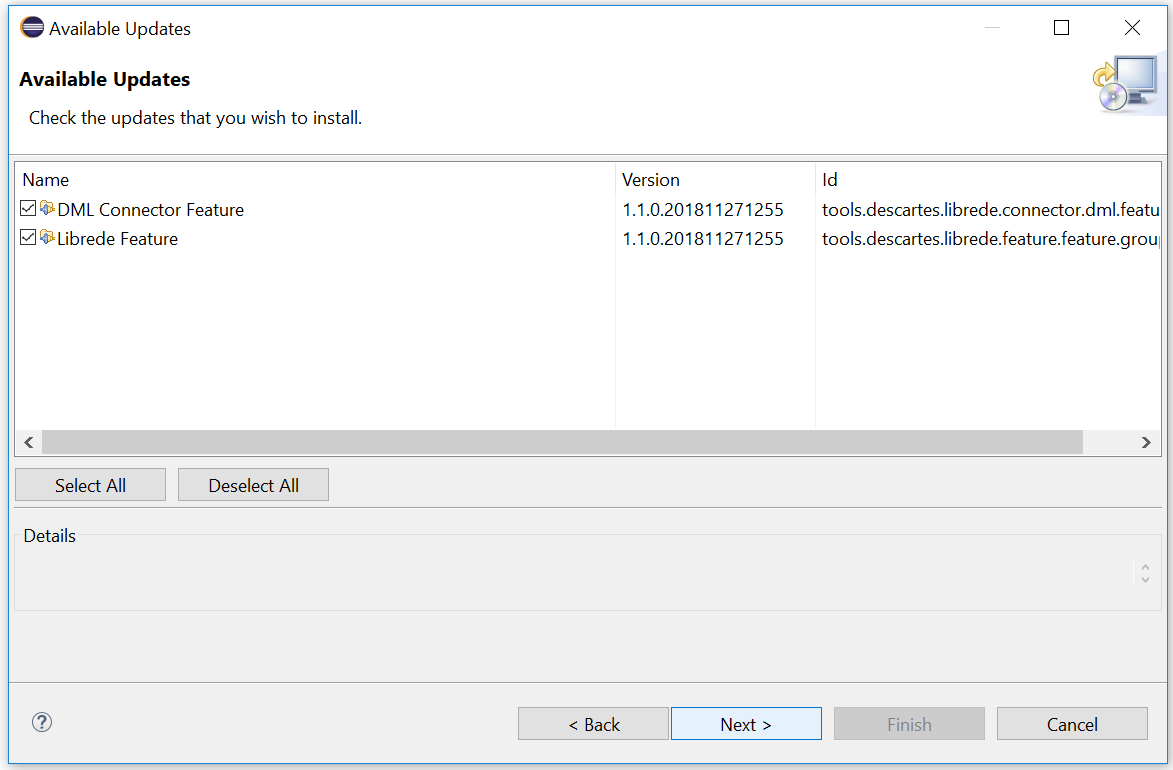
\includegraphics[width=0.9\textwidth]{screenshots/Screenshot8}
			
	\item Accept the license agreement.
	\item Confirm the security warning. \newline
				\newline
				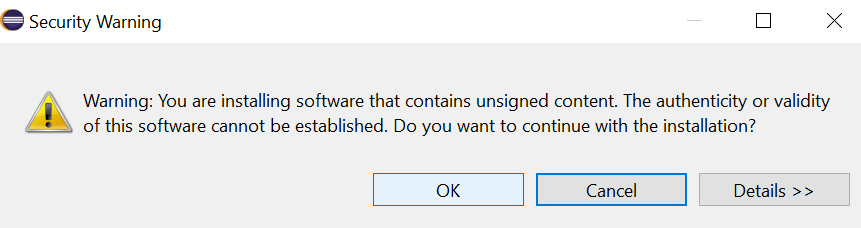
\includegraphics[width=0.6\textwidth]{screenshots/Screenshot6}	
	\item After completion, restart Eclipse. \newline
	
\end{itemize}

\section{Step by Step Example}

This section explains the usage of Librede with a step-by-step example.

\begin{itemize}
	\item Create a new project in your workspace.
	\item Download example files from \url{https://bitbucket.org/librede/librede/downloads/LibredeExamples.zip} and extract the archive to your hard disk.	
	\item Import the measurement traces from the downloaded ZIP archive into your project. \newline
			\newline
			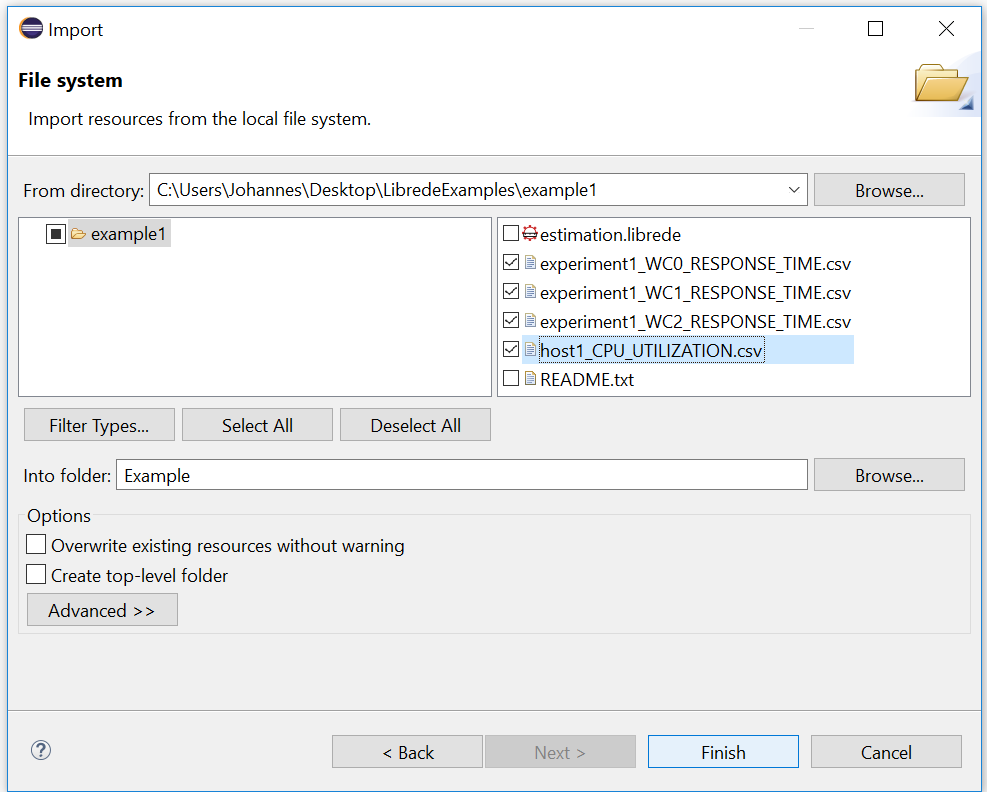
\includegraphics[width=0.6\textwidth]{screenshots/Screenshot9} \newline
	\item Check the structure of the imported measurement traces. The traces are standard CSV files with two or more columns. The first column contains a unix timestamp (counting seconds from 1.1.1970), the second and any other columns contain measurements from a system.
	\newline \newline
			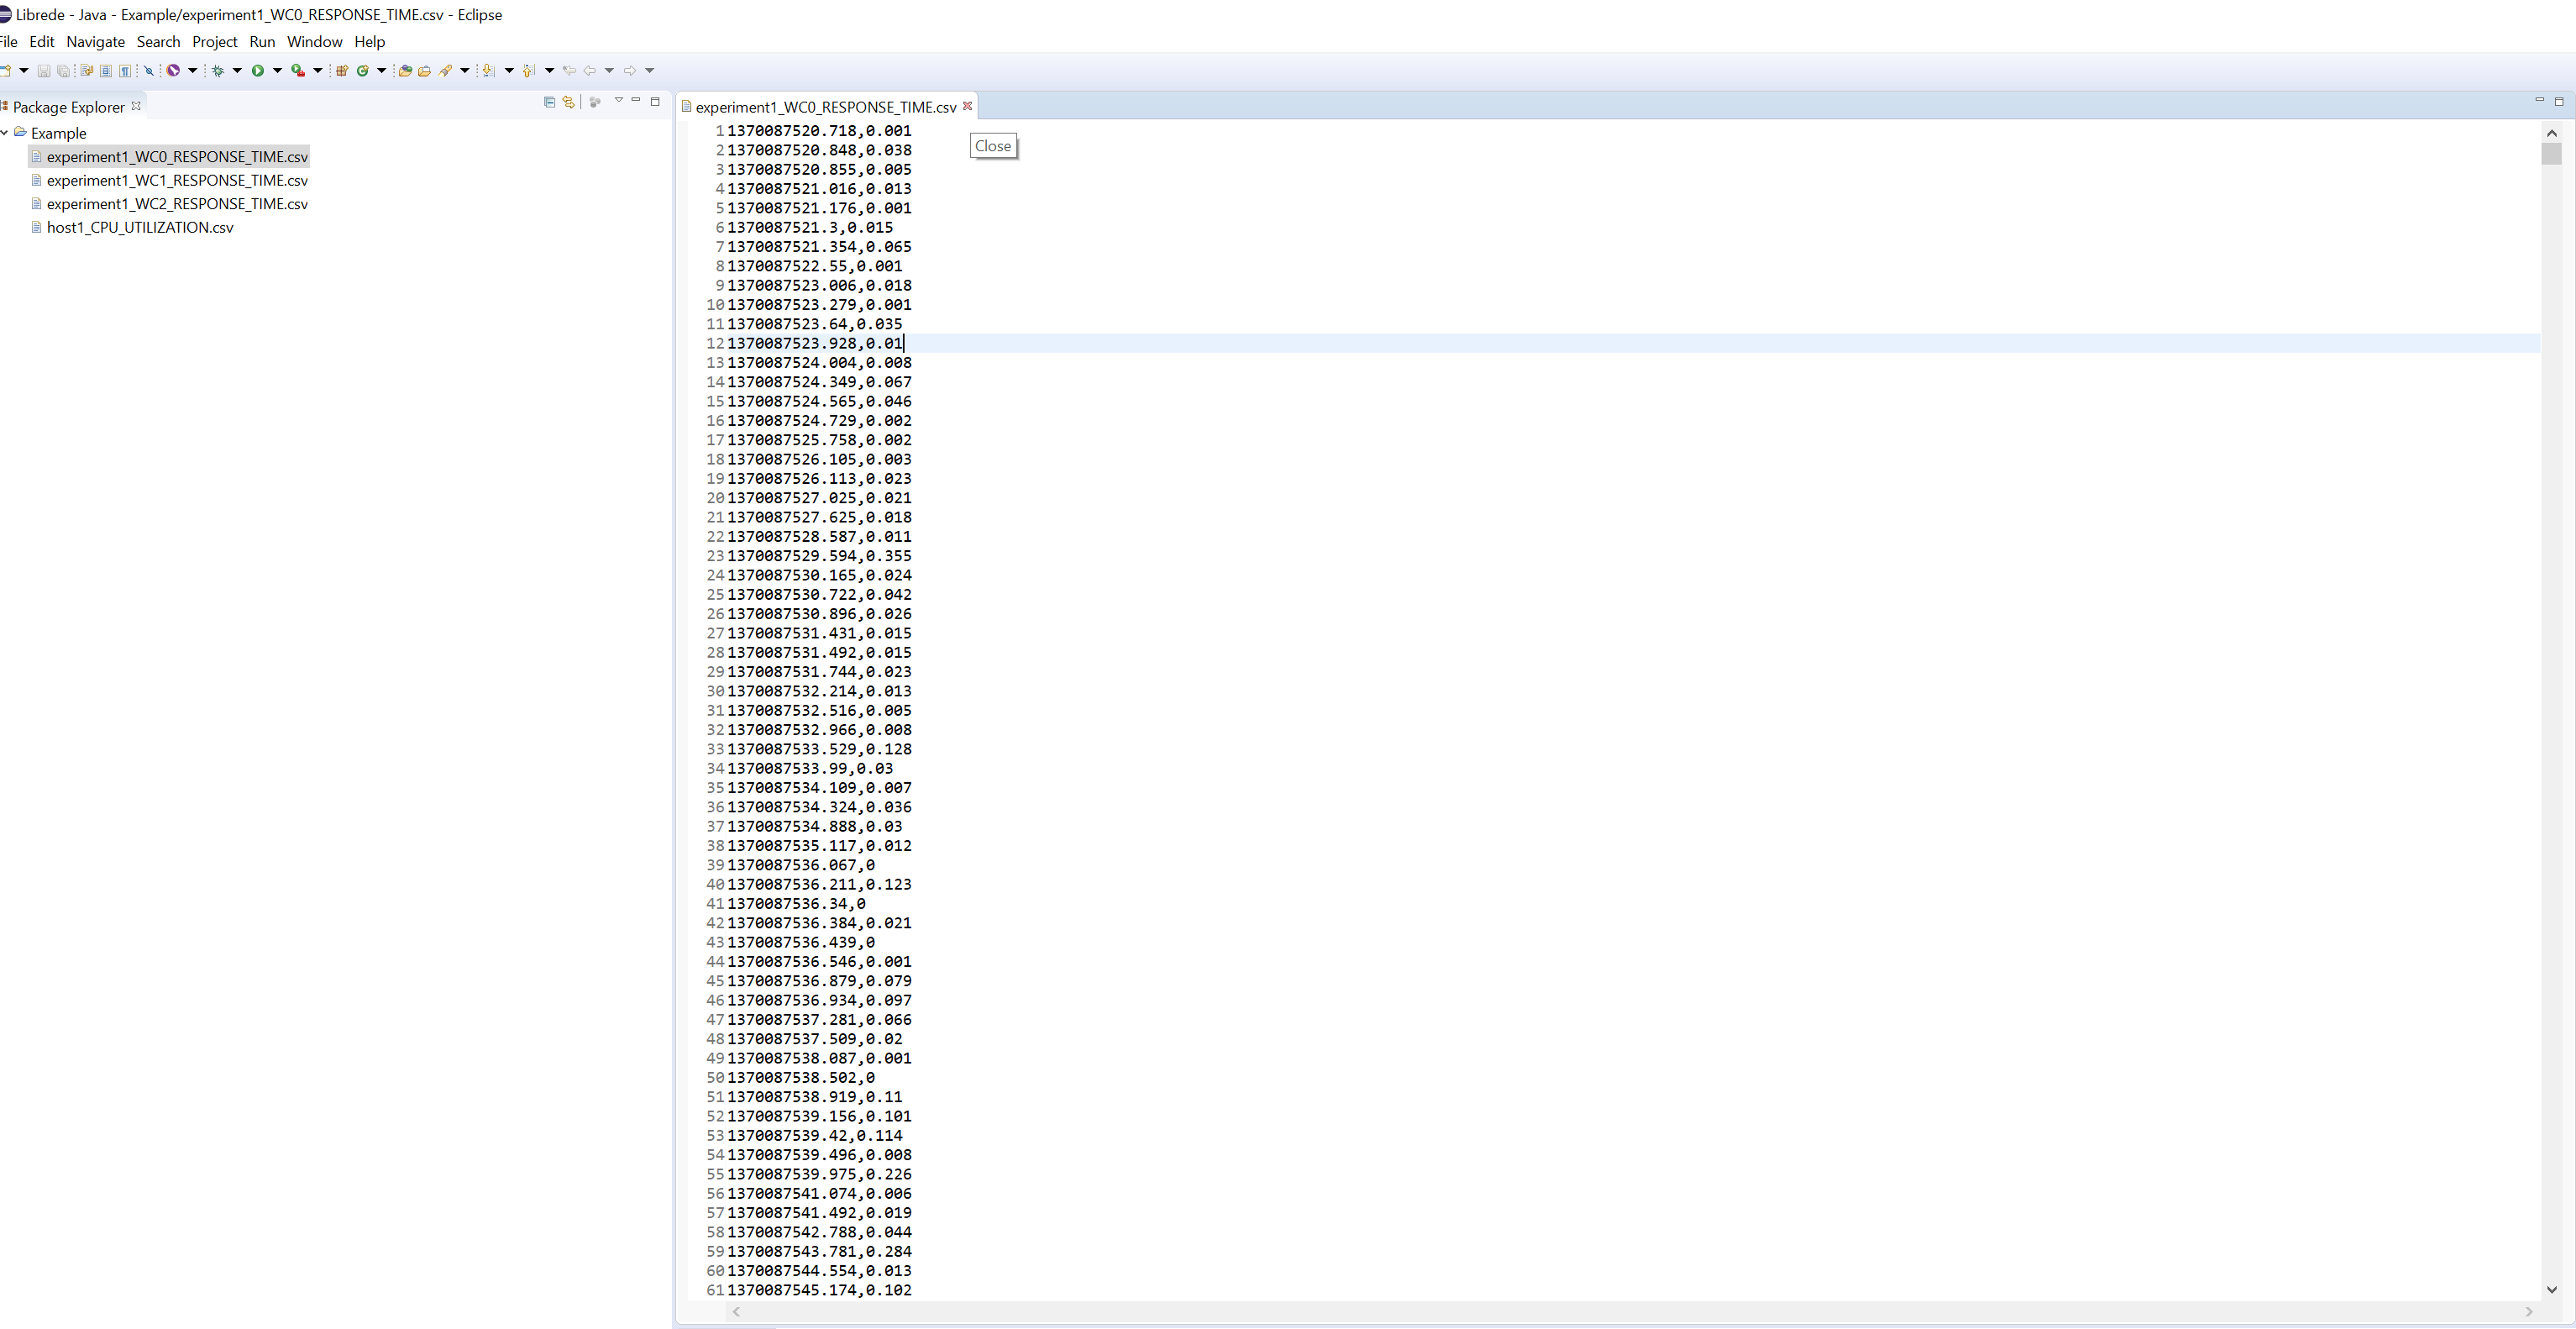
\includegraphics[width=0.9\textwidth]{screenshots/Screenshot10} \newline \newline
			The monitoring data must be available as time series data with associated timestamps for each sample. The library can work on time series with individual events (e.g., arrival times and response times of individual requests) or on fixed sampled time-aggregated data (e.g., average response times or average throughput). If the input data consists of time series with individual events, the library automatically computes the required time-aggregated data. 
	\item Create a new Librede estimation model in this project using the wizard "Librede Estimation Model" (see screenshots below). A complete estimation model can be found in the examples ZIP archive. However, note that the configuration just serves as an example and does not work right away (as the file-paths have to be adapted). Therefore, we will create a new estimation model in the next steps. \newline
				\newline
				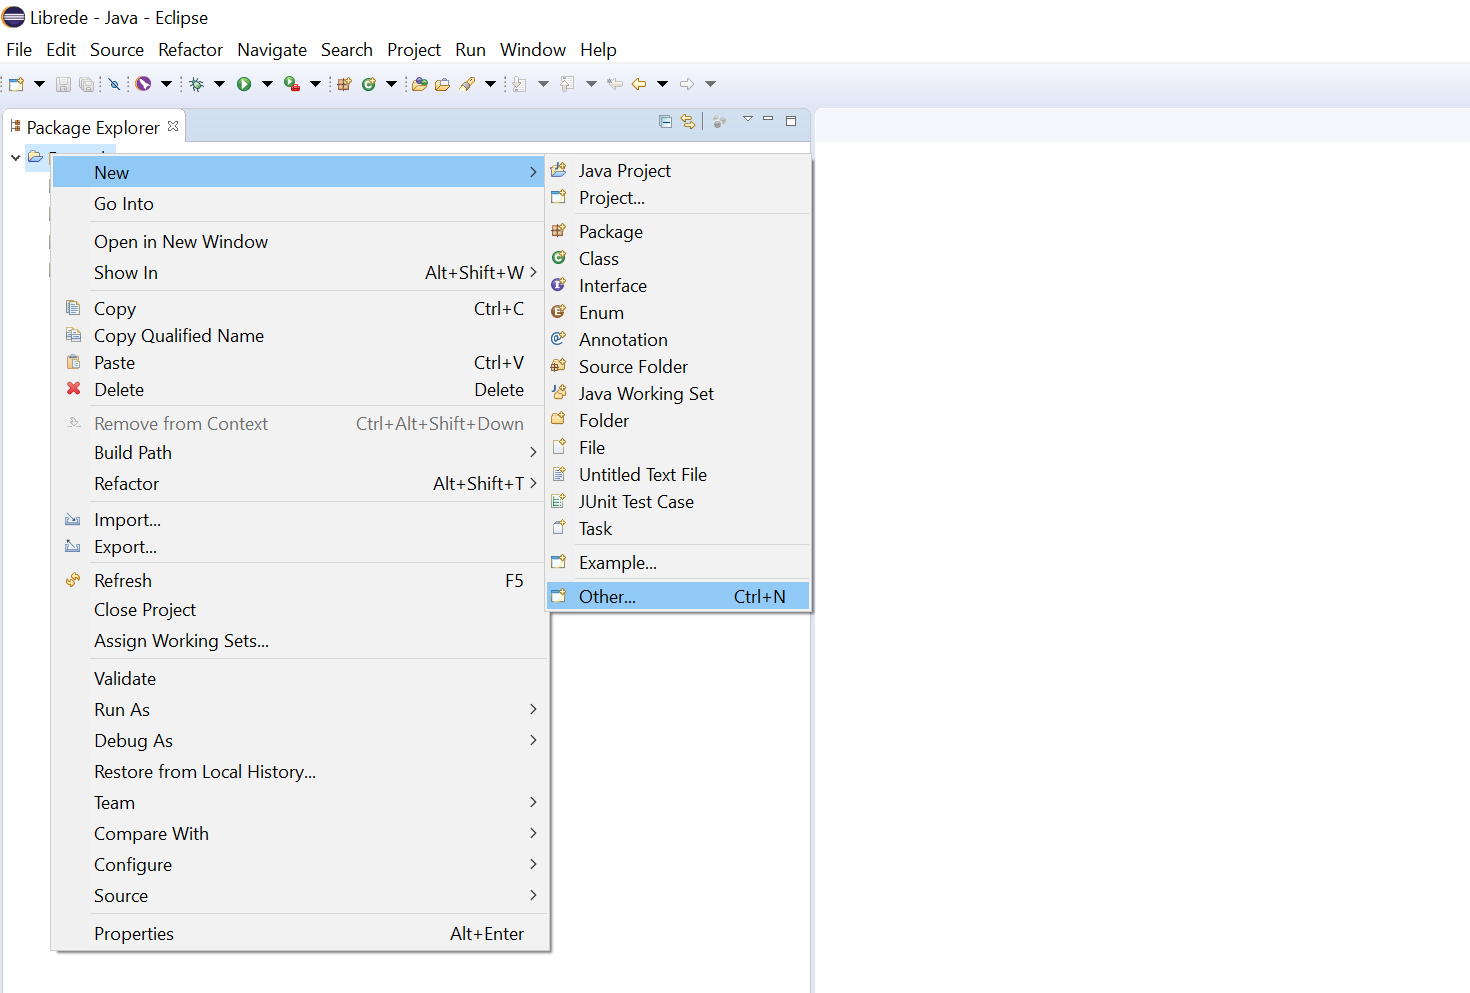
\includegraphics[width=0.9\textwidth]{screenshots/Screenshot11} \newline
				\newline
				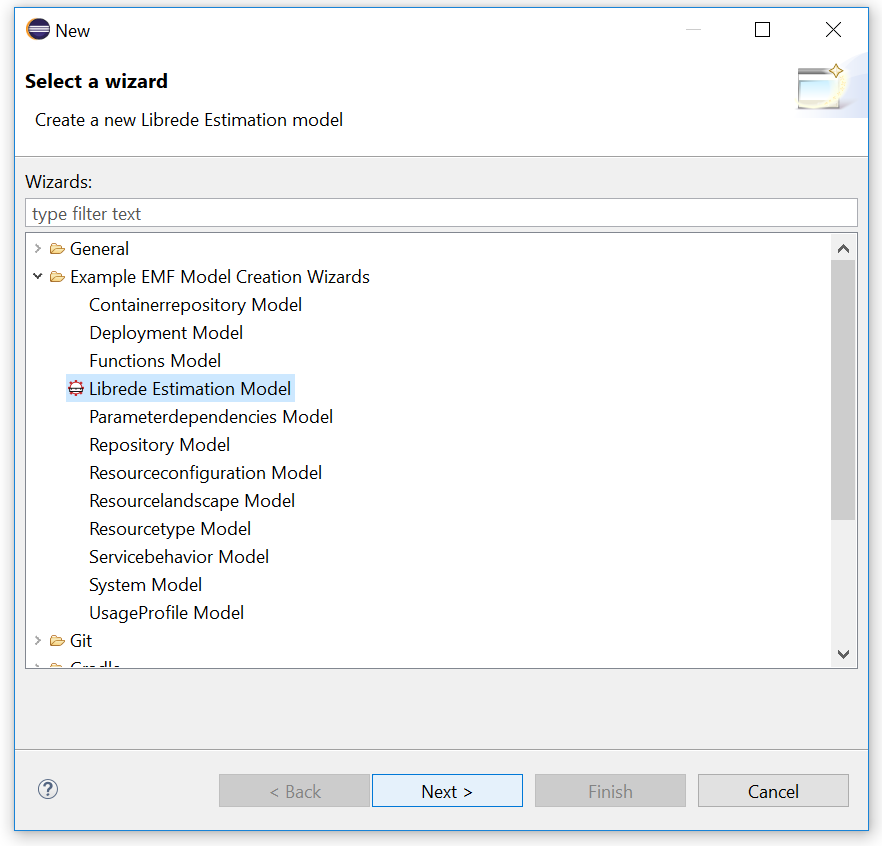
\includegraphics[width=0.6\textwidth]{screenshots/Screenshot12}			
	\item The estimation approaches require a description of the workload of the system under study. The workload description consists of the services (also known as workload classes), which are distinguished during estimation, and the resources for which resource demands will be estimated. Add services WC0, WC1, WC2 and resource Host1 in the workload description. Set number of servers to 1 and the scheduling strategy to "Unkown", as we do not want to make any assumptions on the scheduling strategy.\newline
			\newline
			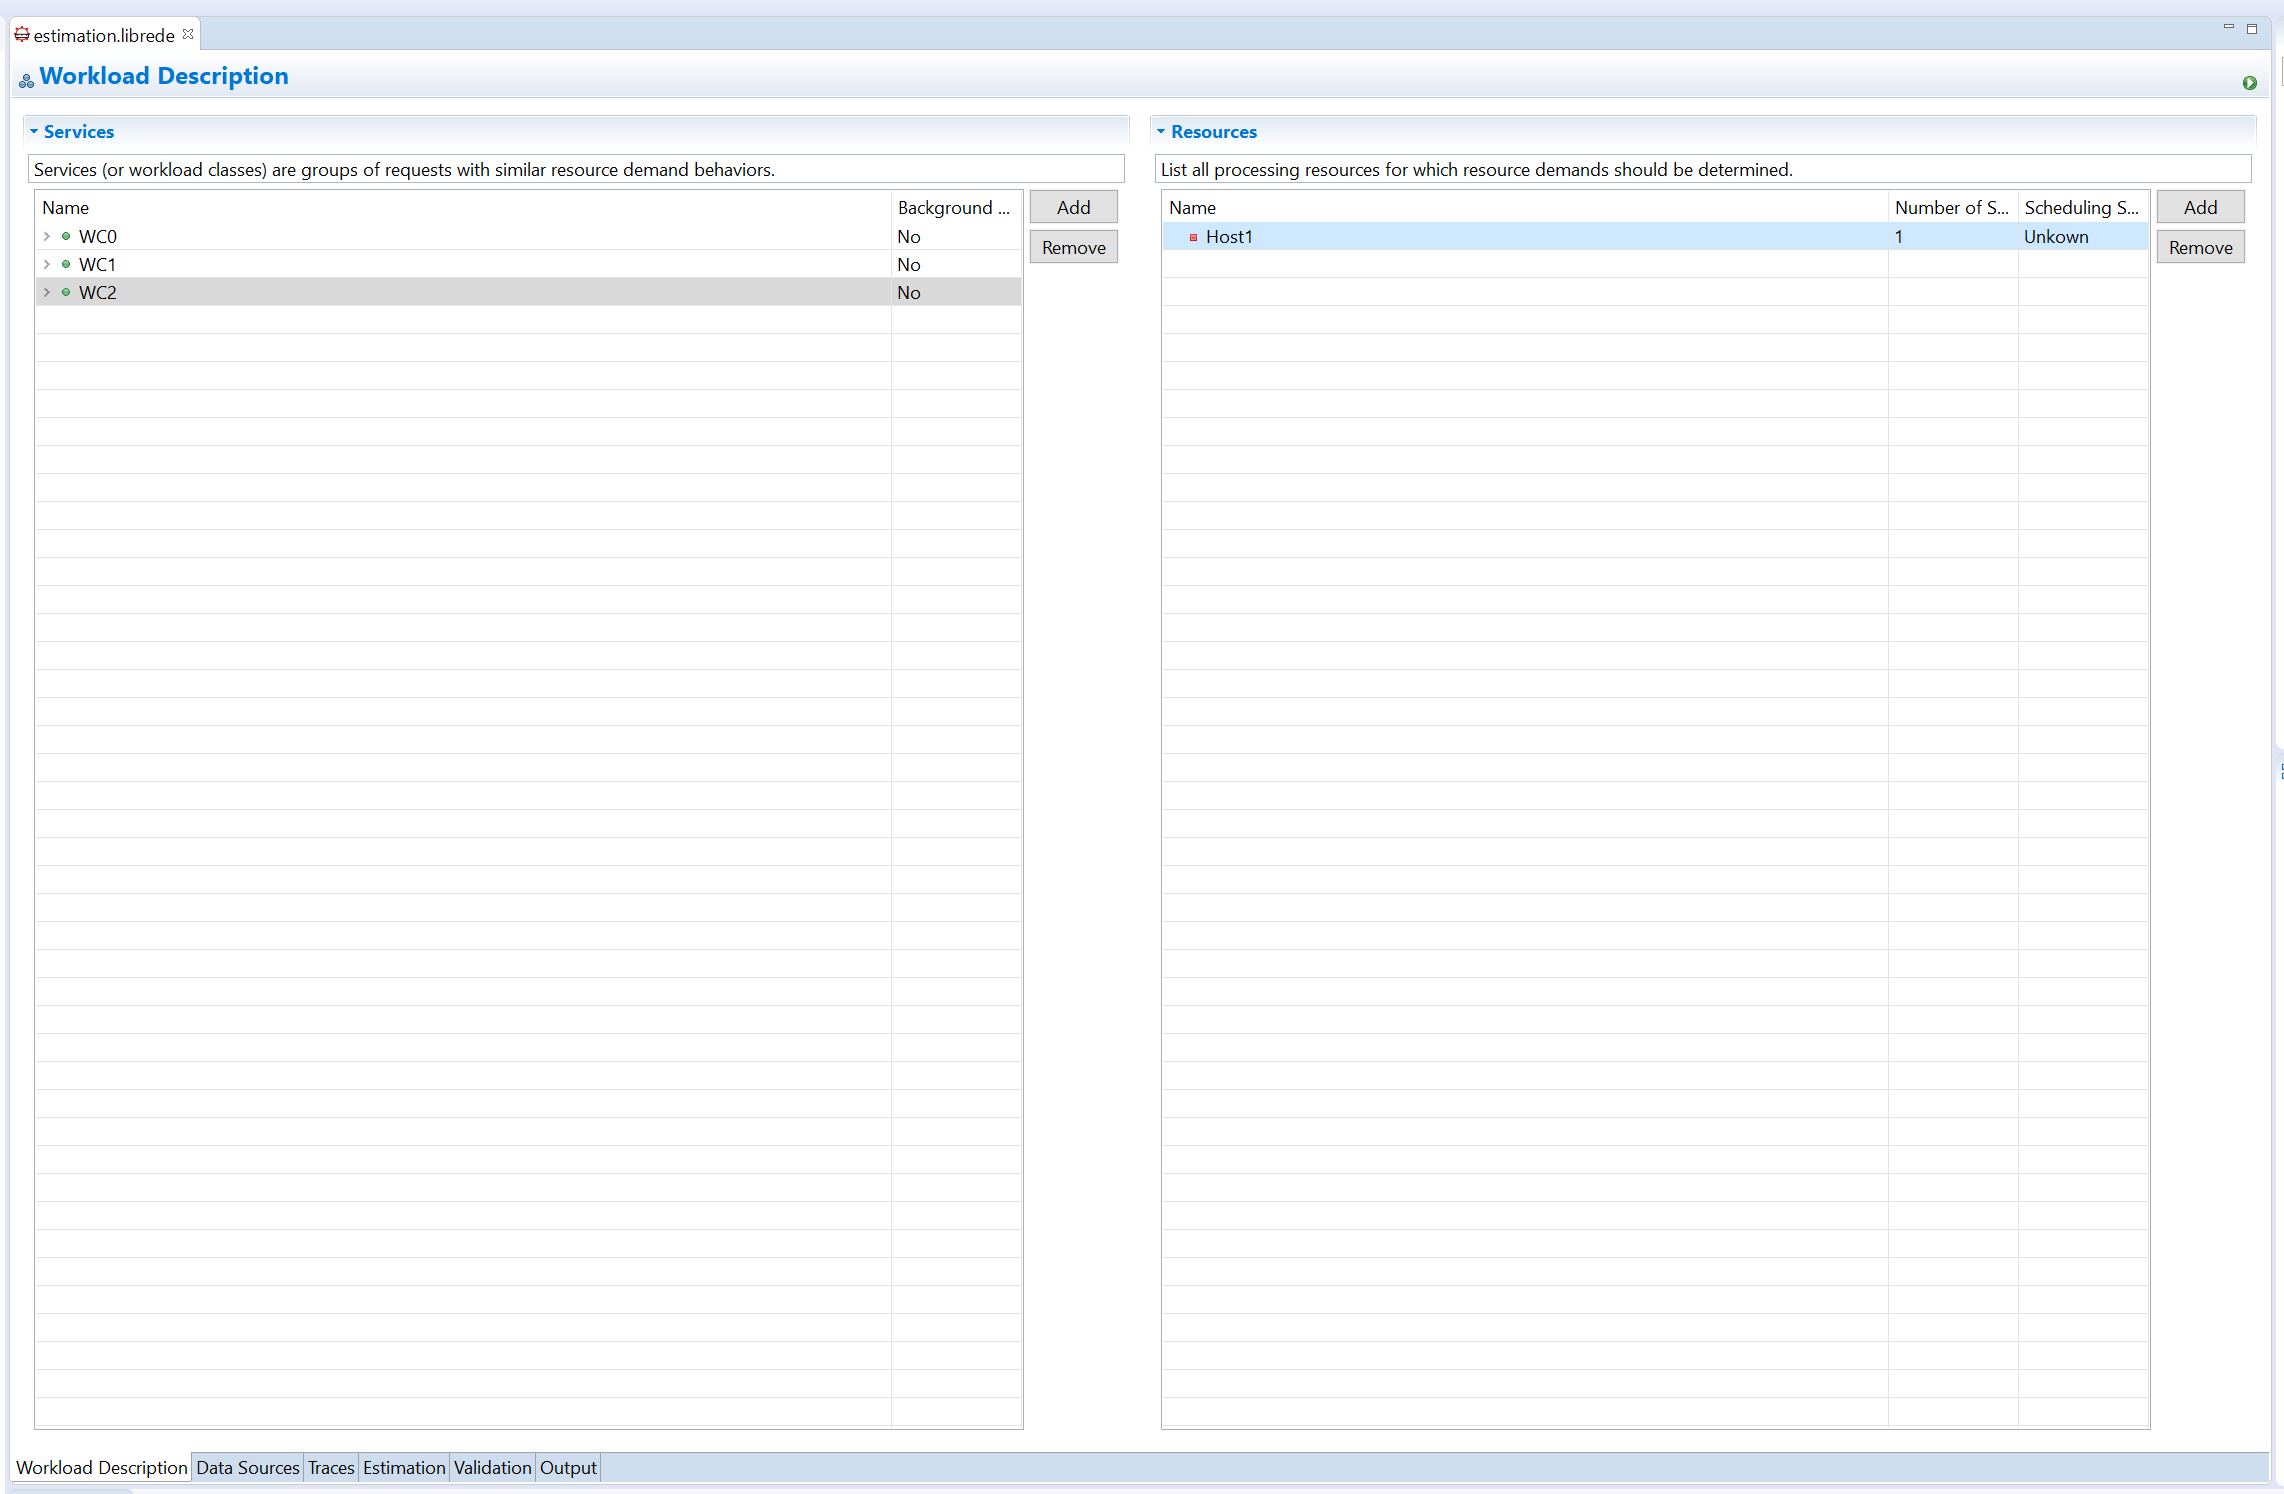
\includegraphics[width=0.9\textwidth]{screenshots/Screenshot13}
	\item Go to page \emph{Data Sources} and add a new datasource with default values. The name property is just for easier identification. The separator char may be changed depending on the format of the CSV files used. \newline
			\newline
			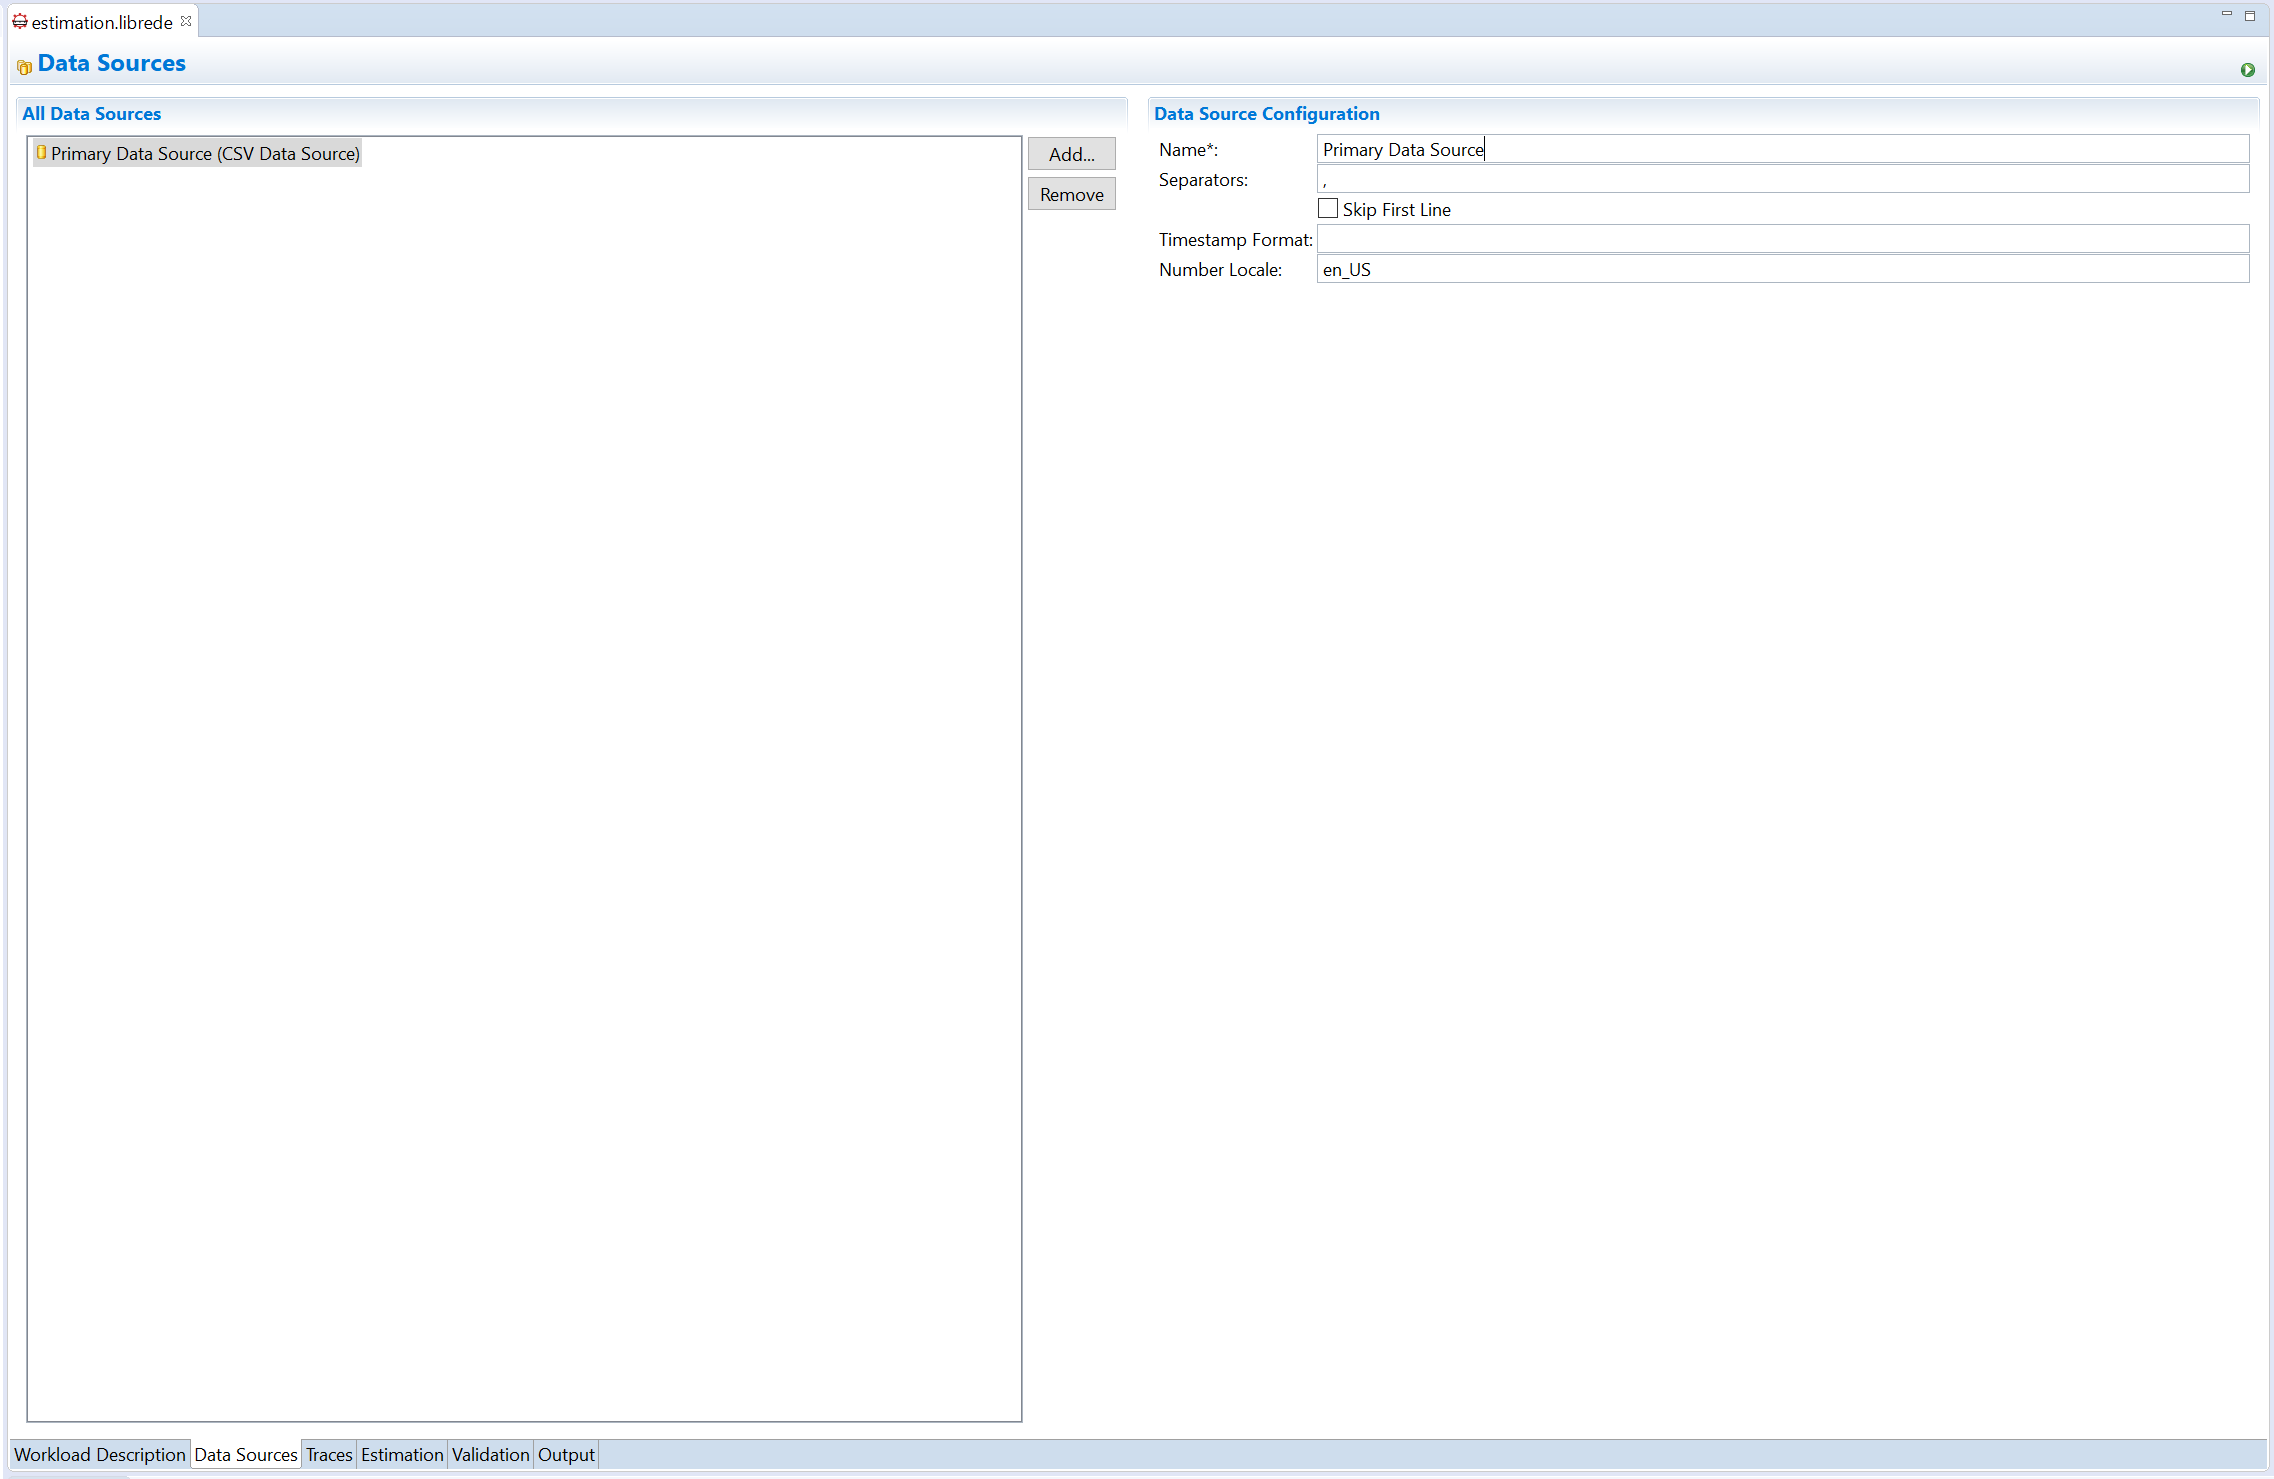
\includegraphics[width=0.9\textwidth]{screenshots/Screenshot14}			
	\item In the next step you define the input measurement traces. Go to page \emph{Traces} in the editor and add a new measurement trace. \newline
			\newline
			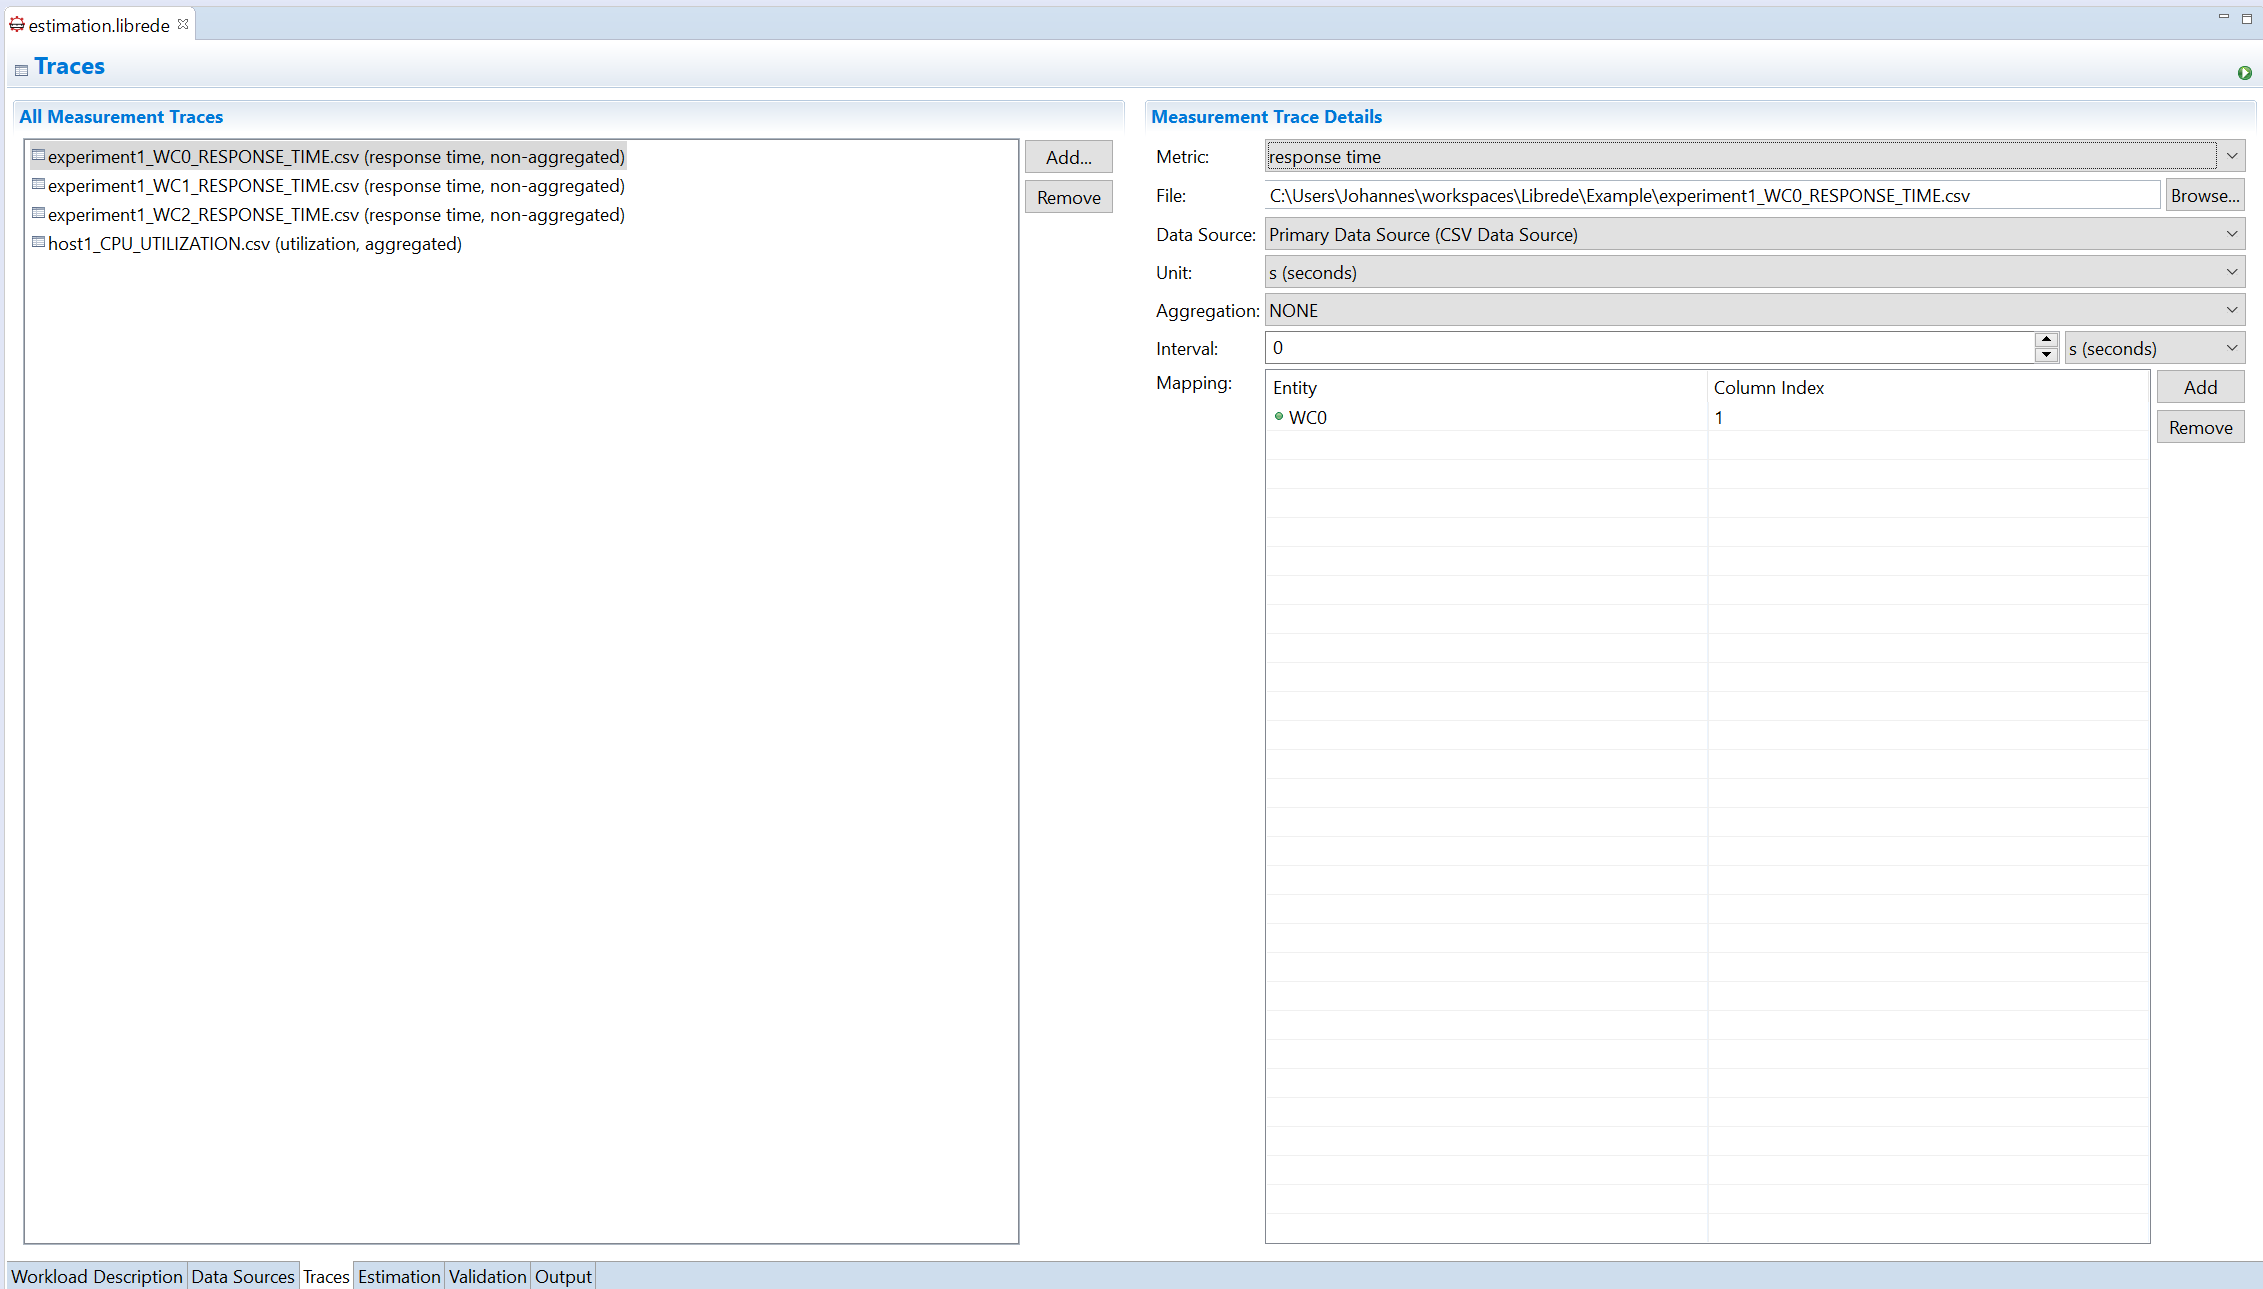
\includegraphics[width=0.9\textwidth]{screenshots/Screenshot26}
			\newline
			Now select the newly created trace and edit the details. Set the \emph{Metric} to ``response time''. For \emph{File}, select the path to "experiment1\_WC0\_RESPONSE\_TIME.csv" in the current project. Select the previously created data source. The measurements are given in seconds, so for \emph{Unit}, we select ``s (seconds)''. Our traces are not aggregated, therefore we set \emph{Aggregation} to ``NONE'' and the interval to 0 seconds. This means that the observations are not aggregated over a time-interval (i.e., in our case we have the response times of individual requests). Then, add a \emph{mapping} to specify the association to service WC0. Column index 1 refers to the first non-timestamp column. Repeat these steps for WC1 and WC2. Make sure, that the other traces map to their corresponding entities (WC1 and WC2, respectively).
			
	\item Next, add a fourth trace describing the CPU Utilization of Host1. Create a new trace with metric "Utilization" and select file "host1\_CPU\_UTILIZATION.csv". 
    \newline
    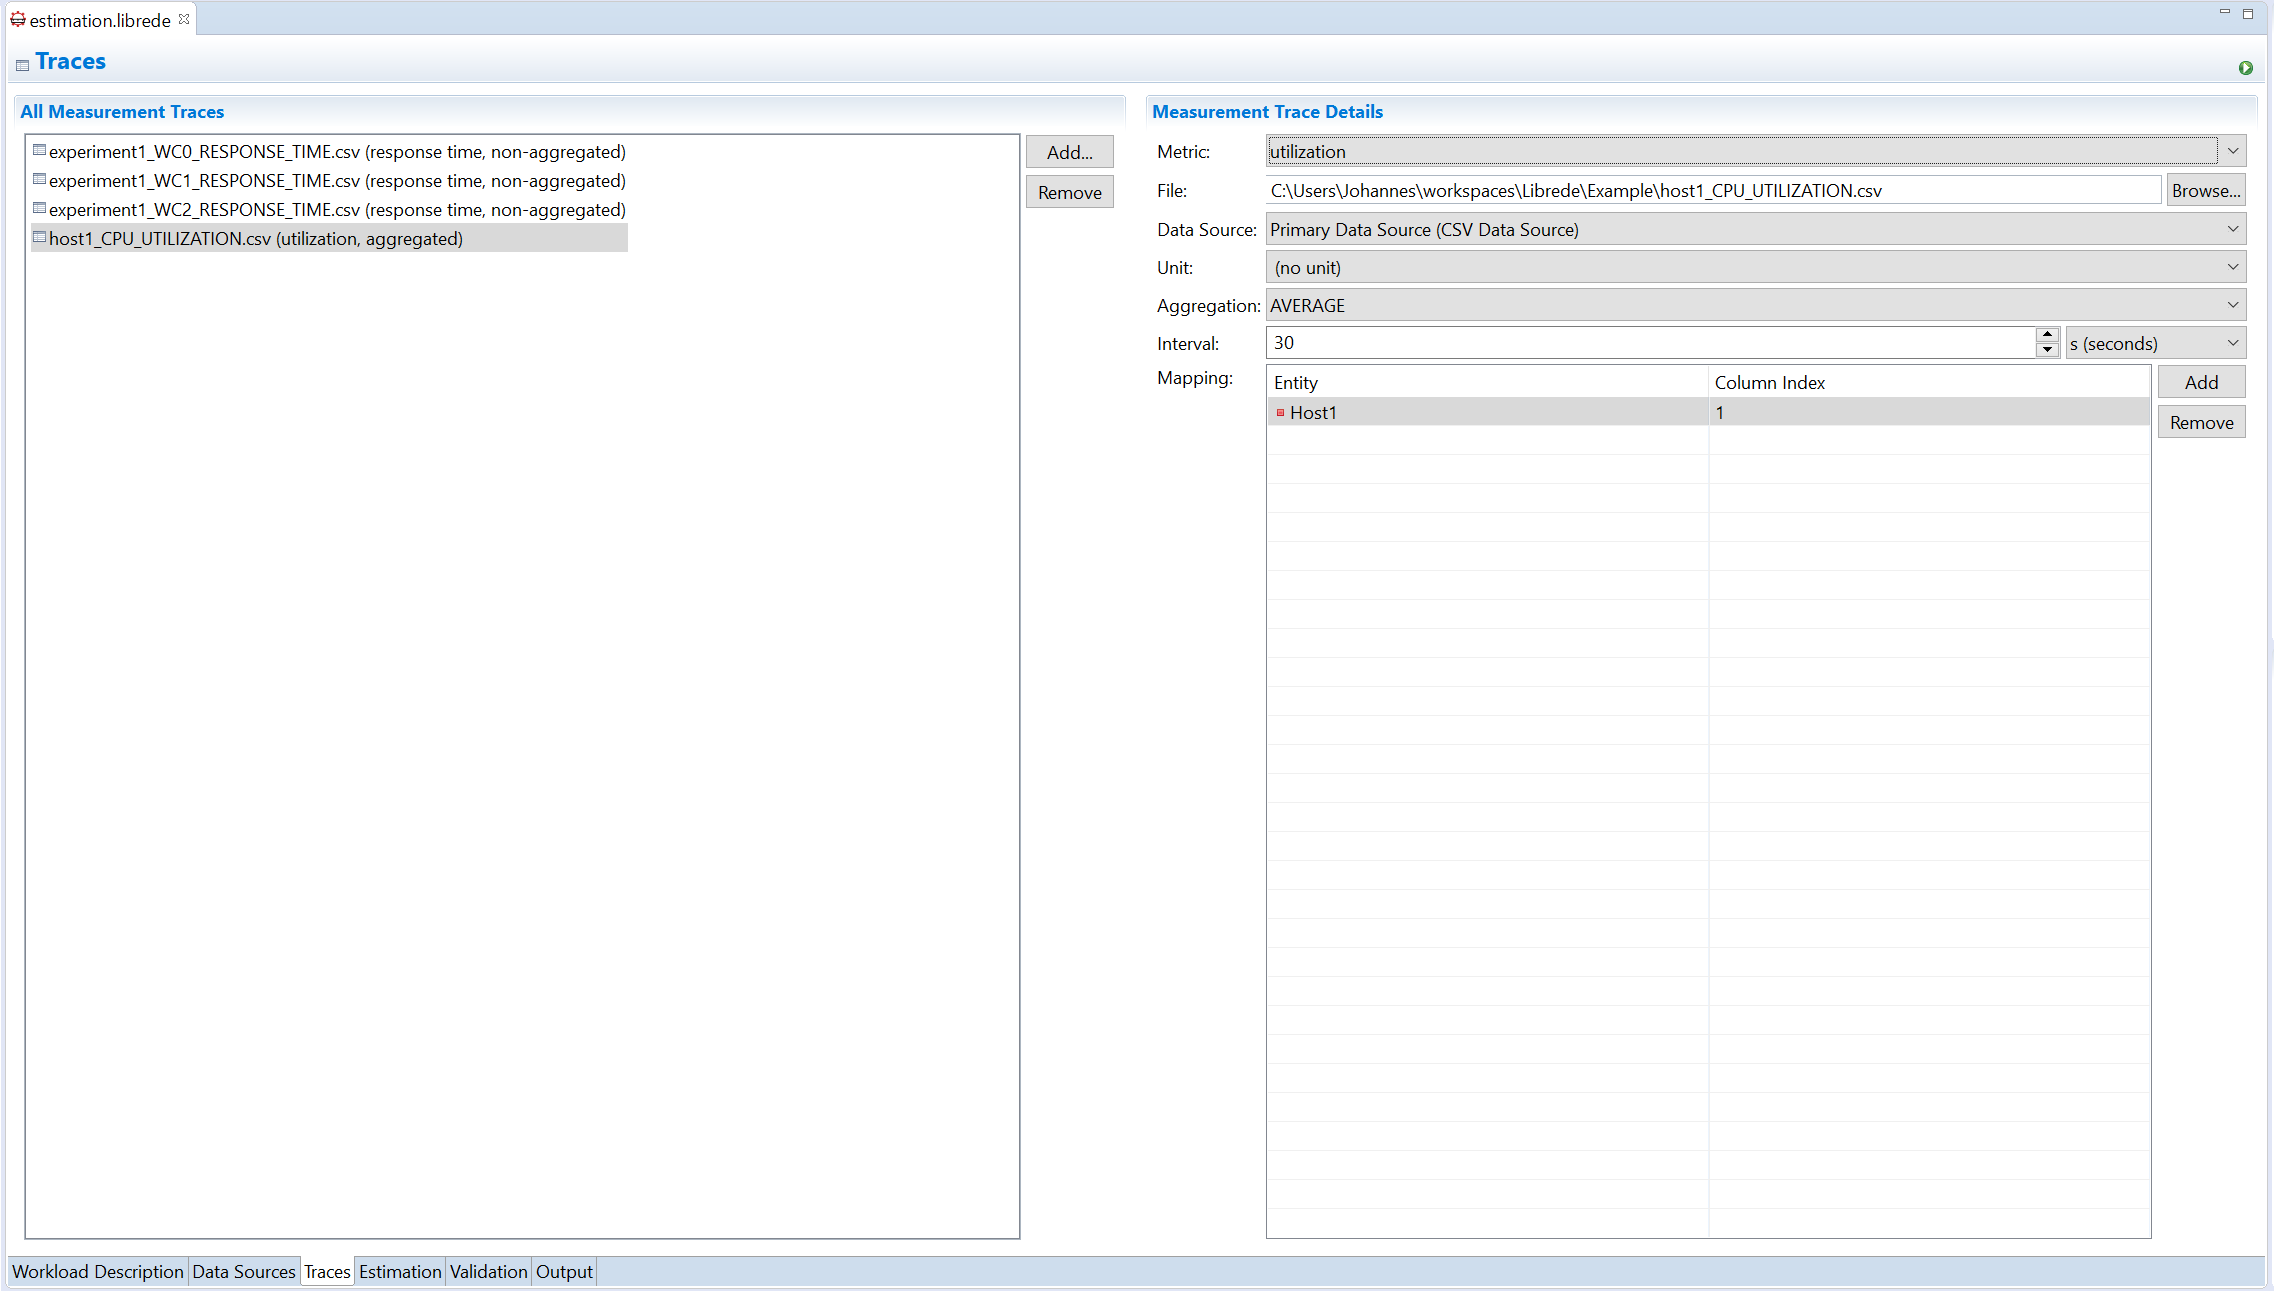
\includegraphics[width=0.9\textwidth]{screenshots/Screenshot25}
    \newline
    We use the same data source as for all other traces. Leave \emph{Unit}' to ``(no unit)'' as the utilization is given as a relative share. Our measurement traces describe the average utilization over the last 30 seconds. Therefore, set the aggregation to ``AVERAGE'' and the interval to 30 seconds. Create a mapping between resource "host1" and column 1.
   
    
	\item Next, switch to page \emph{Estimation} to configure the estimation approach(es) and set the estimation interval.\newline
    
			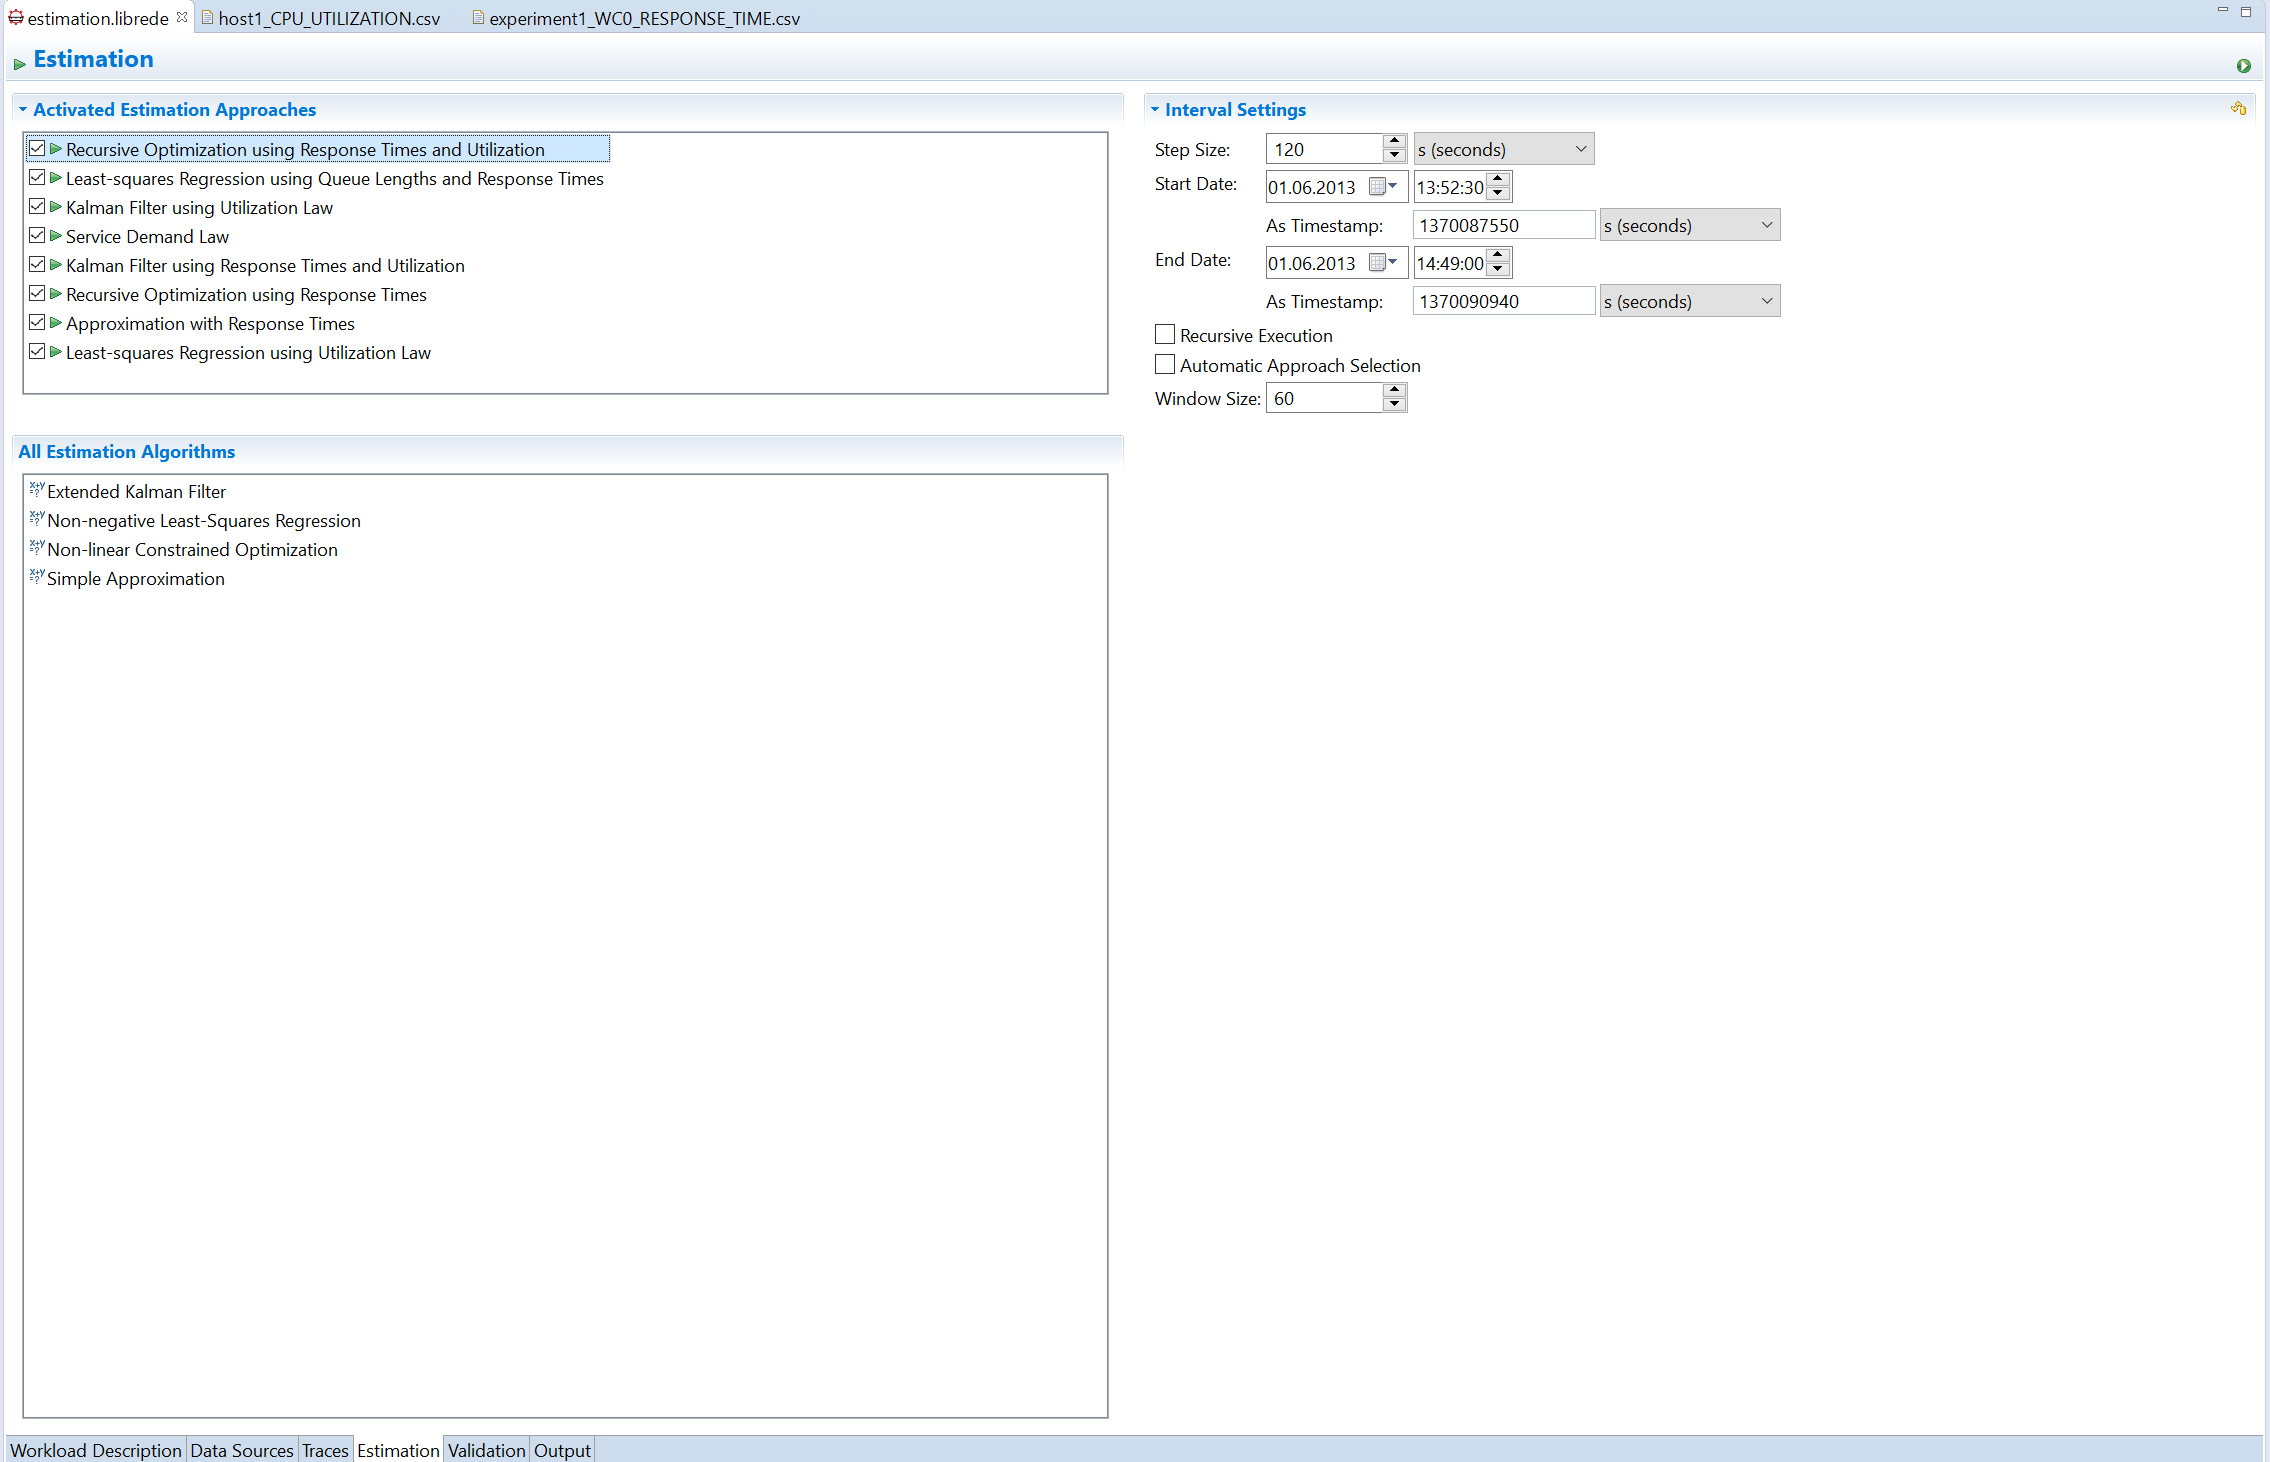
\includegraphics[width=0.9\textwidth]{screenshots/Screenshot19}	 \newline \newline
			The \emph{step} size defines in which interval the estimates are updated. If there are traces with aggregated measurements, the step size must be equals or larger than their aggregation interval. However, the step size should not be too large as this may be result in too few samples for estimation. Use 120 seconds for this example. 
            
            \item The \emph{start date} and \emph{end date} needs to specified based on the timestamps in the input measurement traces. Choose a start date of 01.06.2013 13:52:30 and an end date of 01.06.2013 14:49:00 for our example. 
            Note that these timestamps get converted to unix timestamps (as shown below the dates) according to your local timezone. 
            However, the given timestamps have to match to the timestamps in the measurement traces. The example traces were measured in CEST (UTC+2). Therefore, make sure to adapt the given timestamps to your timezone, or (preferably) just enter the unix timestamps 1370087550 as start and 1370090940 as end date. The date will the adapt accordingly.
			
			\item The \emph{recursive execution} flag determines whether the resource demands at the end of each estimation interval will be written to the output or only the final result. The parameter \emph{window size} can be used to control the maximum number of samples considered for estimation. Set the window size to 60 in the example. 
            The flag \emph{Automatic Approach Selection} automatically analyses the results and recommends the favorable approach. 
            Disable both flags for this example.
			
			
		
	\item 	Check that all estimation approaches are activated. Some of the estimation approaches are configurable to optimize approach-specific parameters. Use the default values here. \newline
			\newline
			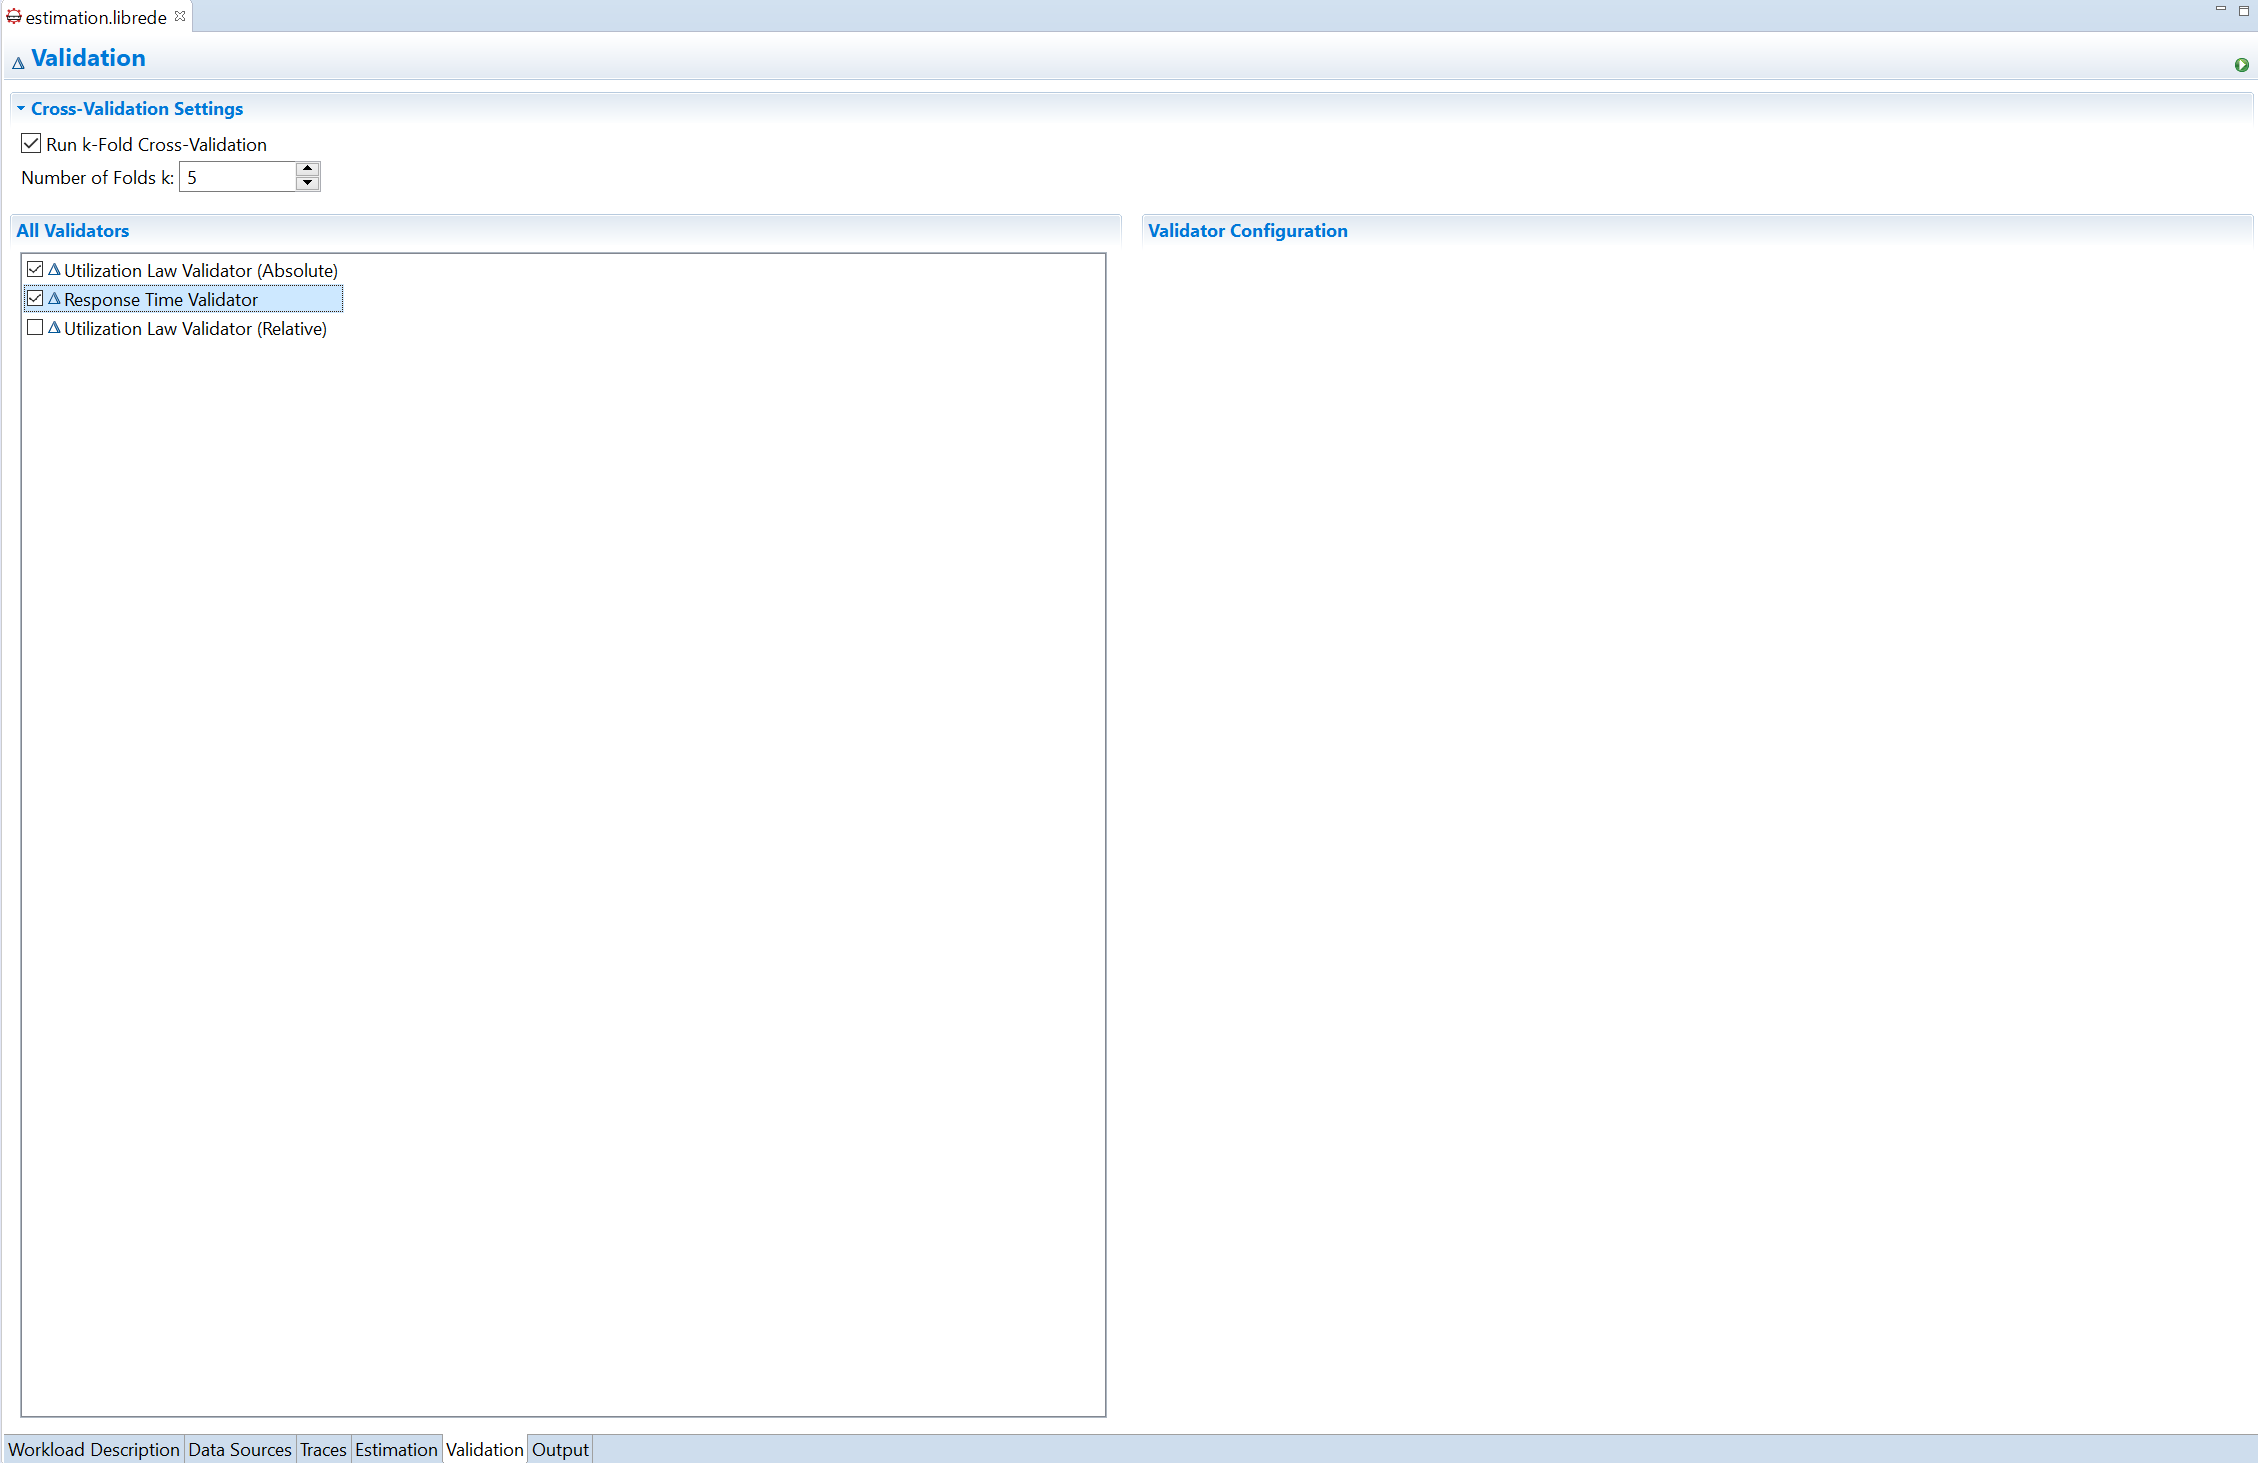
\includegraphics[width=0.9\textwidth]{screenshots/Screenshot21}	
	\item Switch to page \emph{Validation}. Ensure that the $k$-fold Cross-Validation is enabled and set the number of folds to 5. Also, ensure that Response Time Validator and Utilization Law Validator (absolute) are enabled. \newline
			\newline
			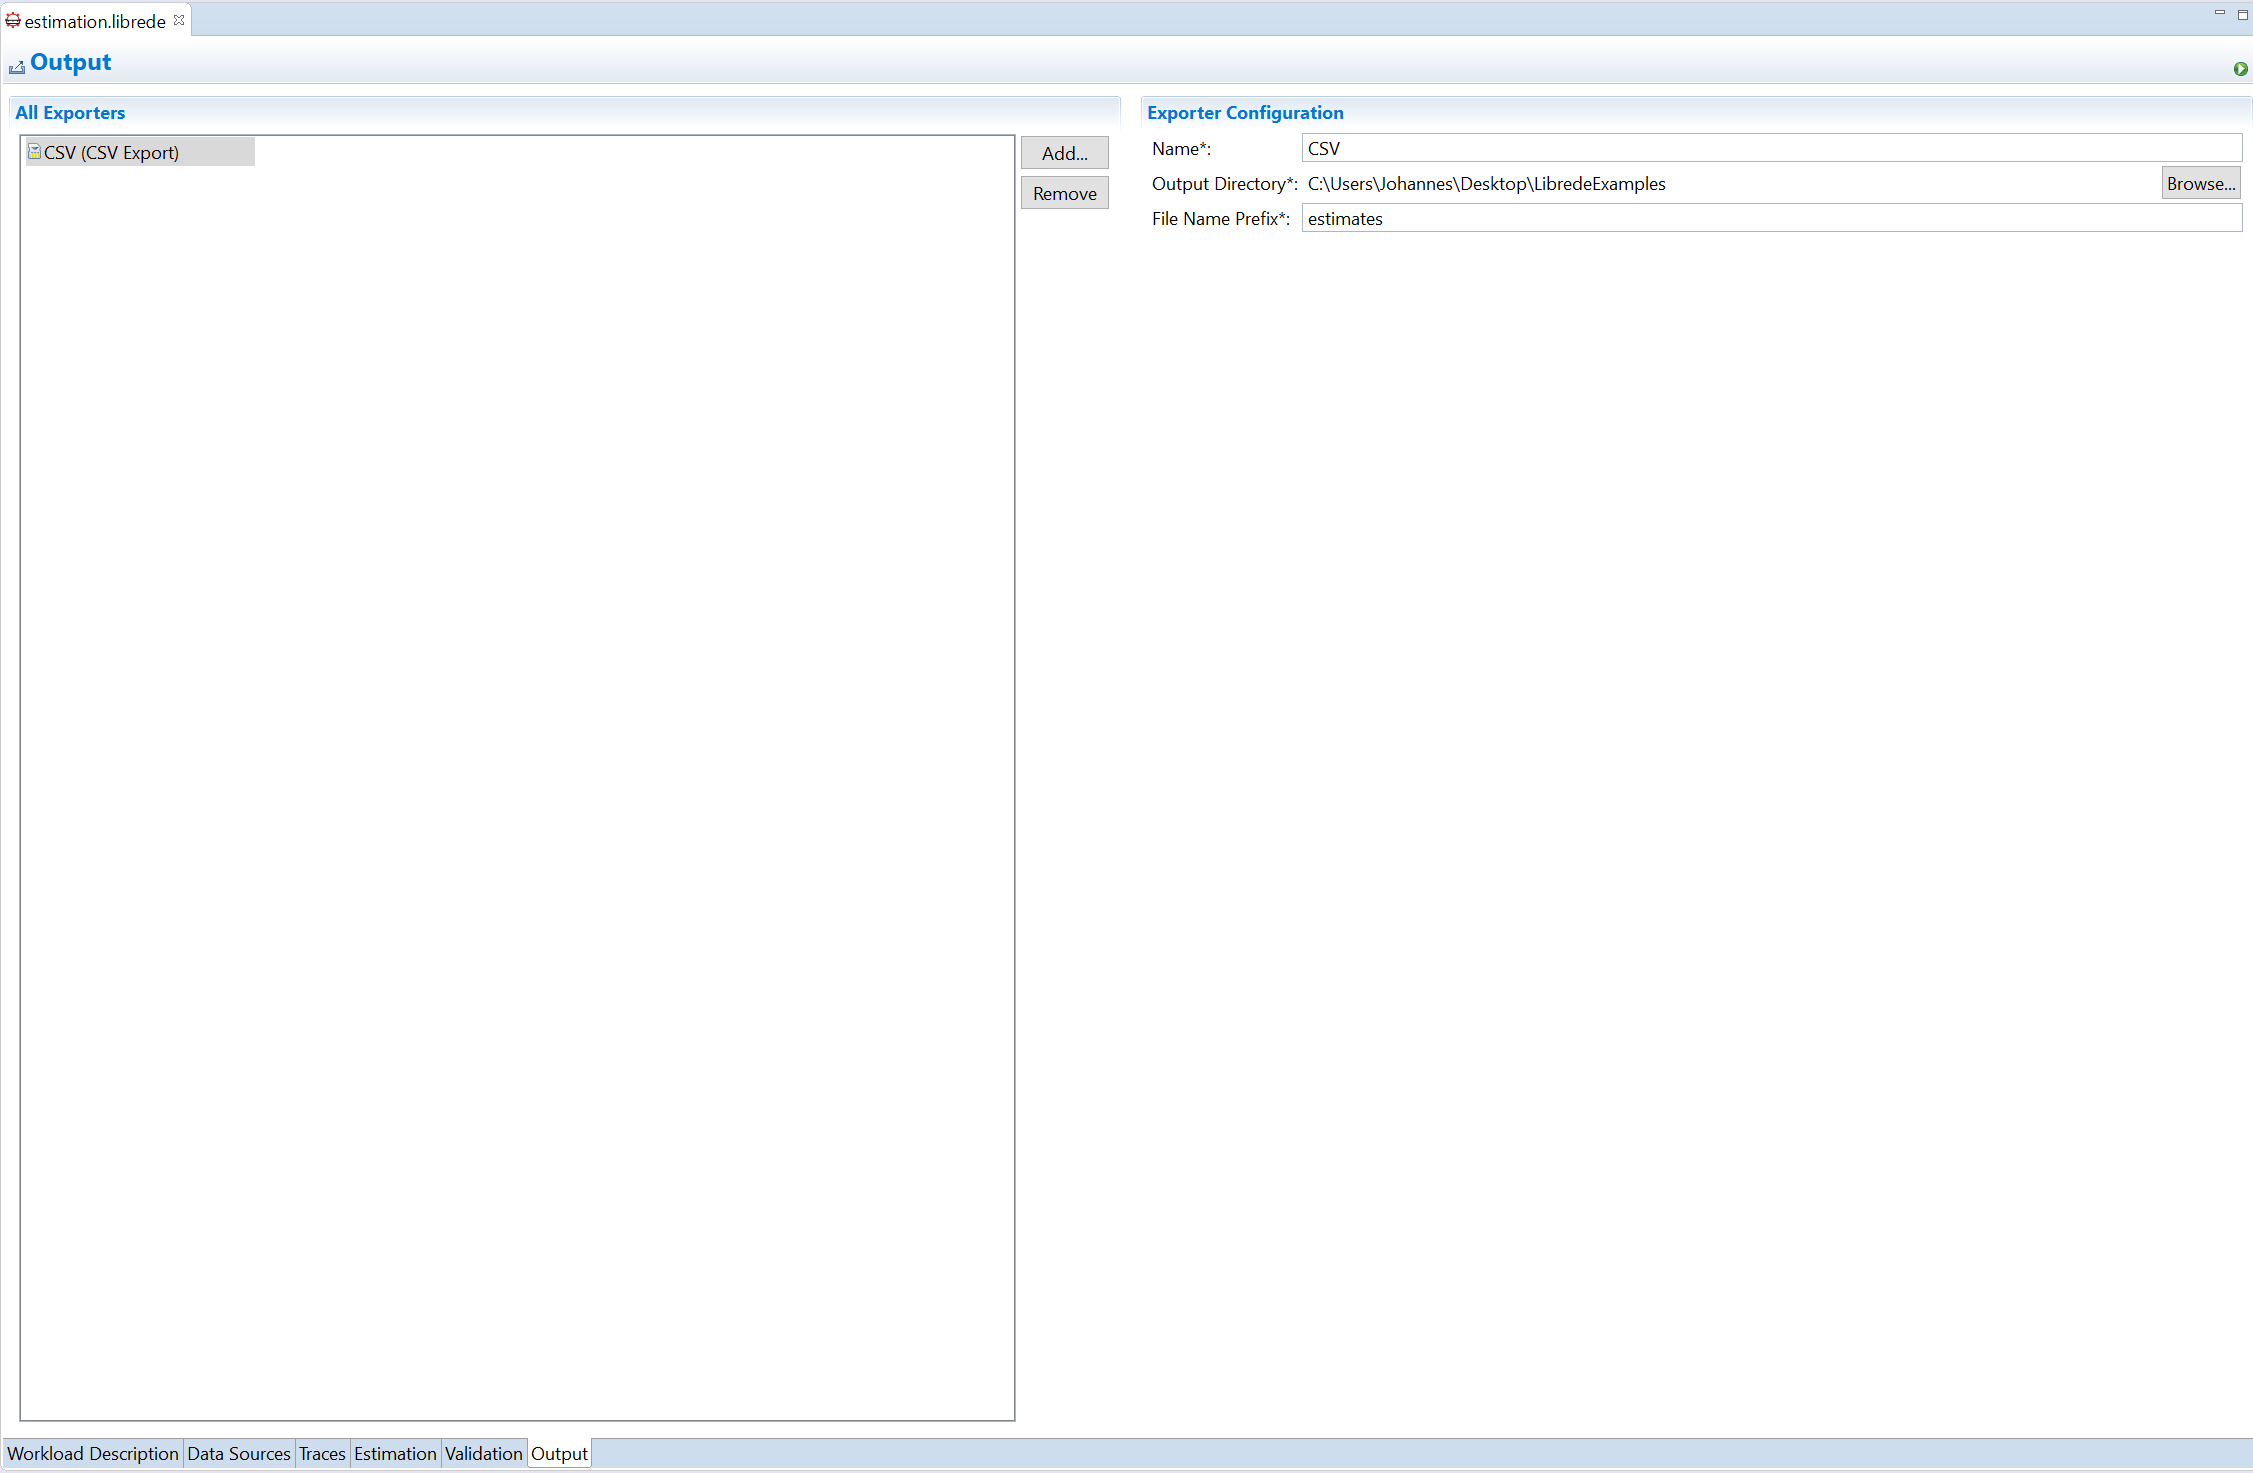
\includegraphics[width=0.9\textwidth]{screenshots/Screenshot23}		
	\item Go to page "Output" to configure the persistency of the results. Add a new CSV export. The \emph{name} property is just for easier identification. Set the \emph{output directory} to a directory of your choice. The value of property \emph{file name prefix} will be prepended to each created output file. Set it to "estimates".
    
     Note: It is not necessary to configure a file output. If you are fine with console output, you can skip this step. \newline	
	\item Start the estimation by clicking the green arrow in the upper right corner of the editor.
	\item The results of the estimation and the cross-validation are printed to the console and the output files. 
    
    Note that your results are probably not identical to the ones shown here. Execution result can differ slightly for every execution. This is due to random selections of the $k$ validation folds and random states of some individual estimators.  \newline
			\newline
			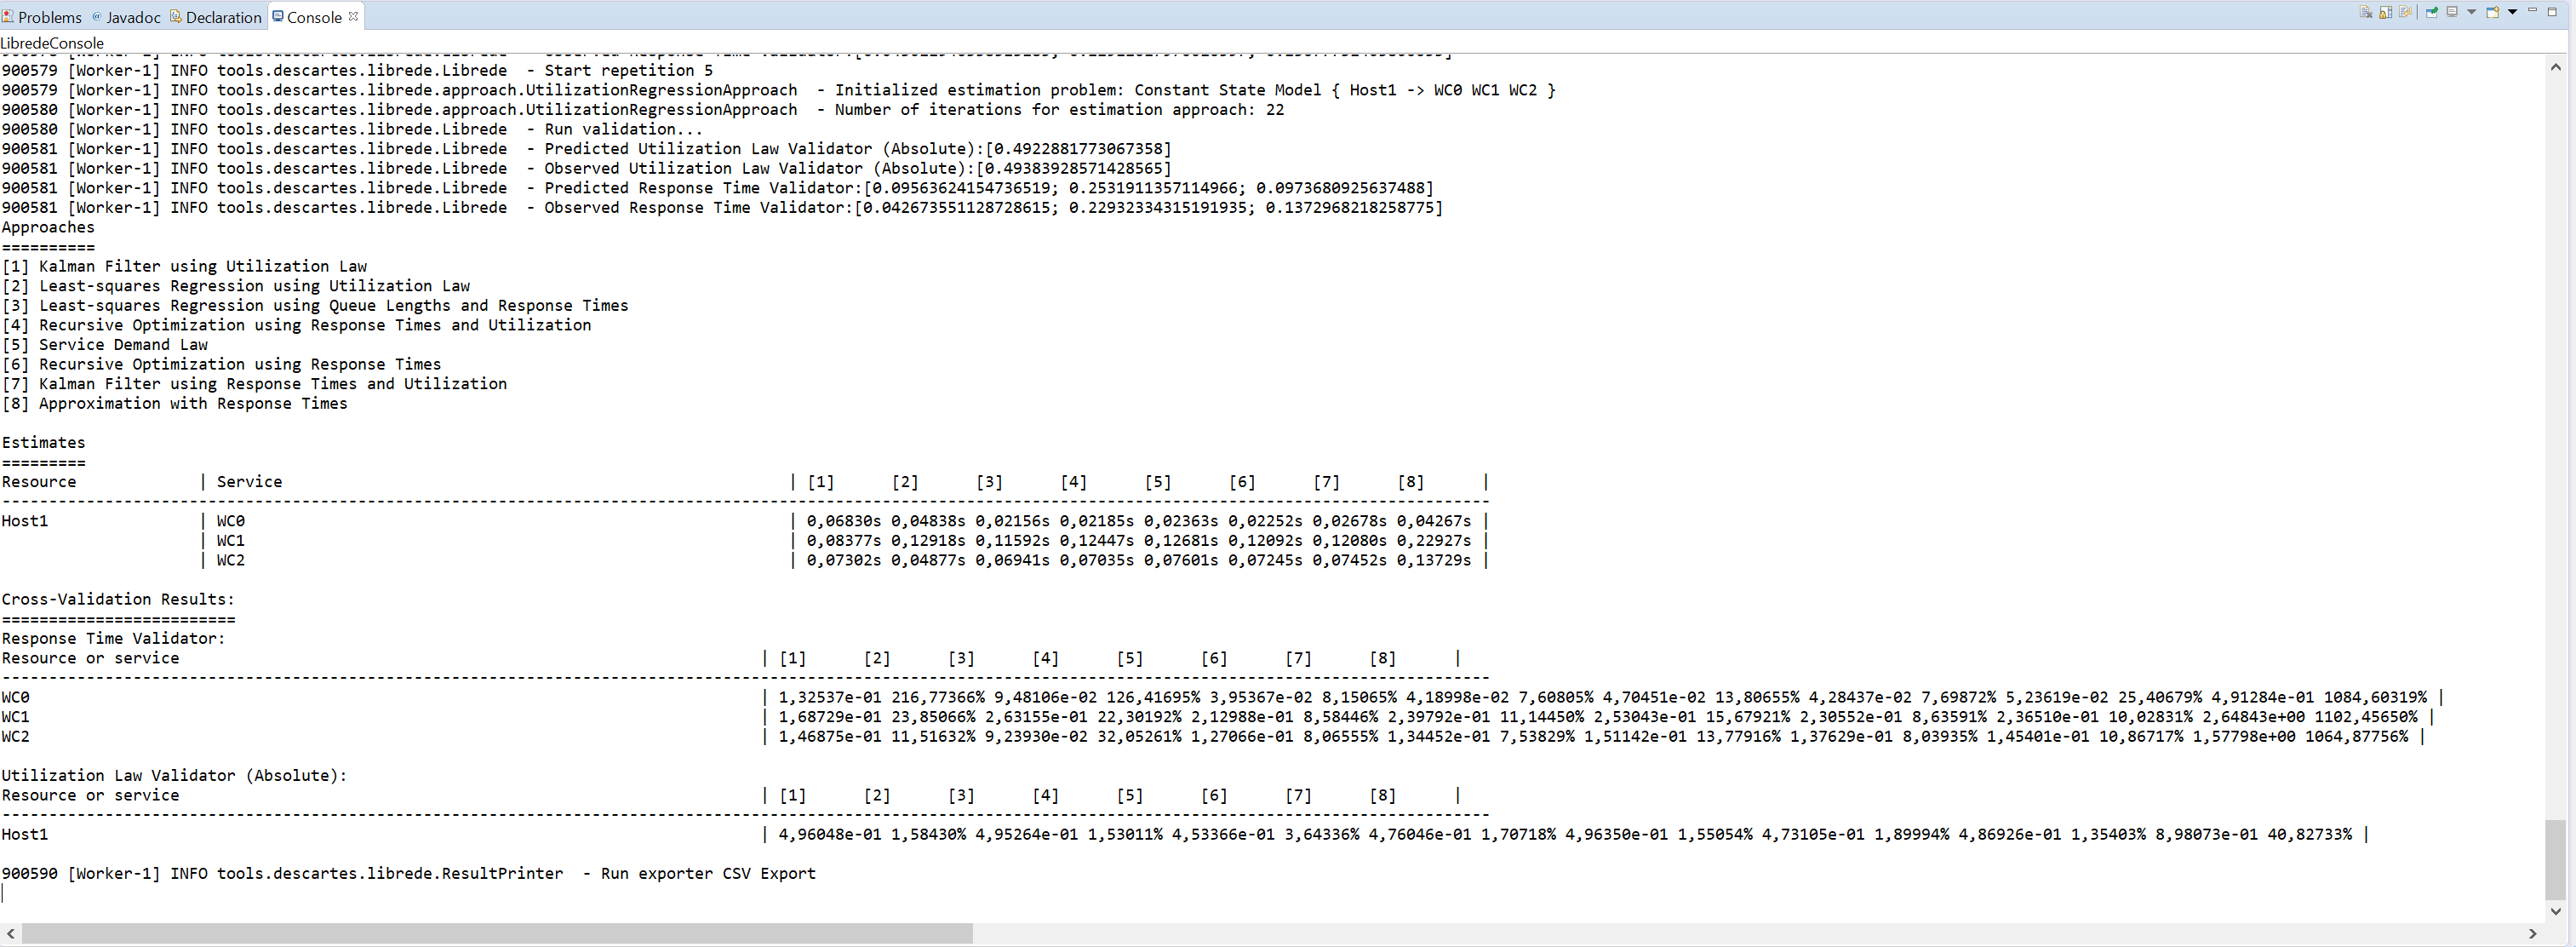
\includegraphics[width=0.9\textwidth]{screenshots/Screenshot27}	\newline
			\newline
			And the generated output-files should be in the folder that you configured previously. \newline
			\newline
	\end{itemize}

\section{Building and Running LibReDE from Console}

It is also possible to run LibReDE from console.
For this, you have to first download and compile the source files it using Maven.
This can be done by the following steps:

\begin{enumerate}
    \item Clone the git repository from Bitbucket: ``git clone https://bitbucket.org/librede/librede.git''
    \item Checkout the development branch: ``git checkout develop''
    \item Switch to the ``tools.descartes.librede.releng'' directory inside the downloaded ``librede'' directory.
    \item Execute the maven packaging: ``mvn clean install -DskipTests''.
    \item Switch to the ``tools.descartes.librede.releng.standalone/target/standalone/console'' directory and execute ``librede.bat'' or ``librede.sh''. You need to provide a valid librede configuration file to be executed.
\end{enumerate}



\section{Calling LibReDE from Java source code}
The main functionality is encapsulated inside the \texttt{Librede} class in the \texttt{tools.descartes.librede} package. 
Here, you have different methods for executing LibReDE. 
The easiest one would be the static method \texttt{execute(LibredeConfiguration conf)}. 
It accepts a \texttt{LibredeConfiguration} as created by the GUI editor. However, this is just an XML-file that has to match the defined EMF-structure and can therefore also manipulated with any standard text editor.
After termination, \texttt{execute(LibredeConfiguration conf)} will return an instance of \texttt{LibredeResults}, containing the estimates along with the error values in the different validation folds.

Any appropriate file can be loaded using the static method \texttt{loadConfiguration(Path path)}. This method tries to load the file on the given path and returns a \texttt{LibredeConfiguration}, if valid. 
The configuration implements a normal object structure.
Therefore, it is also possible to modify or create \texttt{LibredeConfiguration} objects using normal Java commands, since EMF (Eclipse Modeling Framework) was used here.
Its meta-model definition can be found in \texttt{tools.descartes.librede.model}


